%&synopsis-preformat
% ---------------------------------- %
% --- Сборка текста автореферата --- %
% ---------------------------------- %

% --- Служебные пакеты --- %

\RequirePackage[l2tabu, orthodox]{nag} % Вывод информации об используемых пакетах

% --- Определение класса документа --- %

\documentclass[a5paper, 10pt, oneside, openany, article]{memoir}

% --- Подключение общих настроек шаблона, пакетов и команд --- %

% ------------------------------------------------------------------------------ %
% --- Файл упрощённых настроек шаблона, общих для диссертации и автореферата --- %
% ------------------------------------------------------------------------------ %

% --- Режим черновика --- %

\makeatletter
\@ifundefined{c@draft}{
	\newcounter{draft}
    \setcounter{draft}{0} % 0 -- чистовик (максимальное соблюдение ГОСТ)
                          % 1 -- черновик (отклонения от ГОСТ, но быстрая 
                          %       сборка итоговых PDF)
}{}
\makeatother

% --- Пометки в тексте --- %

\makeatletter
\@ifundefined{c@showmarkup}{
	\newcounter{showmarkup}
	\setcounter{showmarkup}{0} % 0 -- скрыть пометки
                               % 1 -- показывать пометки
}{}
\makeatother

% --- Использование в pdflatex шрифтов не по-умолчанию --- %

\makeatletter
\@ifundefined{c@usealtfont}{
  \newcounter{usealtfont}
  \setcounter{usealtfont}{2} % 0 -- шрифты на базе Computer Modern
                             % 2 -- использовать пакет XCharter, 
                             %       при наличии подходящей версии
}{}
\makeatother

% --- Вывод типов ссылок в библиографии --- %

\makeatletter
\@ifundefined{c@mediadisplay}{
	\newcounter{mediadisplay}
    \setcounter{mediadisplay}{1} % 0 -- не делать ничего; надписи [Текст] и
                                 %       [Эл. ресурс] будут выводиться только в ссылках с
                                 %       заполненным полем `media`;
                                 % 1 -- автоматически добавлять надпись [Текст] к ссылкам с
                                 %       незаполненным полем `media`; таким образом, у всех
                                 %       источников будет указан тип, что соответствует
                                 %       требованиям ГОСТ
                                 % 2 -- автоматически удалять надписи [Текст], [Эл. Ресурс] и др.;
                                 %       не соответствует ГОСТ
                                 % 3 -- автоматически удалять надпись [Текст];
                                 %       не соответствует ГОСТ
                                 % 4 -- автоматически удалять надпись [Эл. Ресурс];
                                 %       не соответствует ГОСТ
}{}
\makeatother

% --- Предкомпиляция tikz рисунков для ускорения работы --- %

\makeatletter
\@ifundefined{c@imgprecompile}{
	\newcounter{imgprecompile}
	\setcounter{imgprecompile}{0} % 0 -- без предкомпиляции;
                                  % 1 -- пользоваться предварительно
                                  %       скомпилированными pdf вместо генерации
                                  %       заново из tikz
}{}
\makeatother
    % Общие настройки шаблона
% ---------------------------------------------------------------------- %
% --- Пакеты, которые являются общими для диссертации и автореферата --- %
% ---------------------------------------------------------------------- %

% --- Логические условия --- %

\newif\ifsynopsis     % Условие, проверяющее, что документ является авторефератом
\usepackage{etoolbox}
\providebool{presentation}

% --- Комментирование текста --- %

\usepackage{comment}    

% --- Поля и разметка страницы --- %

\usepackage{pdflscape} % Для включения альбомных страниц
\usepackage{geometry}  % Для последующего задания полей

% --- Математические пакеты --- %

\usepackage{amsthm, amsmath, amscd} % Математические дополнения от AMS
\usepackage{amsfonts, amssymb}      % Математические дополнения от AMS
\usepackage{mathtools}              % Добавляет окружение multlined
\usepackage{xfrac}                  % Красивые дроби
\usepackage{upgreek}                % Русская традиция начертания греческих букв

% --- Кодировки и шрифты --- %

% Кириллица в нумерации subequations
\patchcmd{\subequations}{\def\theequation{\theparentequation\alph{equation}}}
{\def\theequation{\theparentequation\asbuk{equation}}}
{\typeout{subequations patched}}{\typeout{subequations not patched}}

% Установки для размера шрифта 14 pt
\newlength{\curtextsize}
\newlength{\bigtextsize}
\setlength{\bigtextsize}{13.9pt}
\makeatletter
\setlength{\curtextsize}{\f@size pt}
\makeatother

% Решение проблемы копирования текста в буфер кракозябрами
\ifnumequal{\value{usealtfont}}{0}{}{
    \input glyphtounicode.tex
    \input glyphtounicode-cmr.tex %from pdfx package
    \pdfgentounicode=1
}
    
% Улучшенный поиск русских слов в полученном pdf-файле
\usepackage{cmap}   
\ifnumequal{\value{usealtfont}}{2}{}{
    \defaulthyphenchar=127  % Если стоит до fontenc, то переносы
                            % не впишутся в выделяемый текст при
                            % копировании его в буфер обмена
}

% Дополнительные текстовые символы
\usepackage{textcomp}

% Языковые пакеты
\usepackage[T1, T2A]{fontenc}        % Поддержка русских букв
\usepackage[utf8]{inputenc}          % Кодировка utf8
\usepackage[english, russian]{babel} % Языки: русский, английский

% Подключение русифицированных шрифтов XCharter
\ifnumequal{\value{usealtfont}}{2}{
	\usepackage[scaled = 0.914]{XCharter} 
	%\usepackage[charter, vvarbb, scaled = 1.048]{newtxmath}
	\ifpresentation
	\else
		\setDisplayskipStretch{-0.078}
	\fi
}{}

% --- Оформление абзацев --- %

% Красная строка после заголовков типа chapter
\ifpresentation
\else
    \indentafterchapter
    \usepackage{indentfirst}
\fi

% --- Цвета --- %

\ifpresentation
\else
    \usepackage[dvipsnames, table, hyperref]{xcolor}
\fi

% --- Таблицы --- %

\usepackage{threeparttable} % Автоматическая ширина подписи таблицы
\usepackage{tabularray}     % Таблицы с гибкими настройками

% --- Общее форматирование --- %

\usepackage{soulutf8} % Поддержка переносоустойчивых подчёркиваний и зачёркиваний

% --- Оптимизация расстановки переносов и длины последней строки абзаца --- %

\usepackage[hyphenation, lastparline]{impnattypo}

% --- Работа со списками --- %

\ifpresentation
\else
	\usepackage{enumitem}
\fi

% --- Векторная графика --- %

\usepackage{stanli}   % Отрисовка конструкций
\usepackage{tikz}     % Пакет векторной изображений 
\usepackage{pgfplots} % Построение векторных графиков

% Пакеты Tikz
\usetikzlibrary{shadows}     				% Тени
\usetikzlibrary{arrows.meta} 				% Стрелки
\usetikzlibrary{positioning} 				% Позиционирование 
\usetikzlibrary{calc}        				% Расчетная библиотека
\usetikzlibrary{trees} 		 				% Построение деревьев
\usetikzlibrary{external}	 				% Компиляция изображений
\usetikzlibrary{decorations.pathreplacing}  % Изменения отображения пути
\usetikzlibrary{calligraphy}  				% Каллиграфия
\usetikzlibrary{angles}						% Отображение углов
\usetikzlibrary{patterns}					% Штриховка

% --- Гиперссылки --- %

\usepackage{color}
\usepackage{hyperref}

% --- Изображения --- %

\usepackage{graphicx}   % Подключаем пакет работы с графикой
\usepackage{caption}    % Подписи рисунков и таблиц
\usepackage{subcaption} % Подписи подрисунков и подтаблиц
\usepackage{pdfpages}   % Добавление внешних pdf файлов
\usepackage{float}      % Дополнительные опции размещения

% --- Счётчики --- %

\usepackage{aliascnt}                  % Псевдонимы счетчиков
\usepackage[figure, table]{totalcount} % Счётчик рисунков и таблиц
\usepackage{totcount}                  % Пакет создания счётчиков на основе последнего номера
                                       %  подсчитываемого элемента (может требовать дважды
                                       %  компилировать документ)
\usepackage{totpages}                  % Счётчик страниц, совместимый с hyperref (ссылается
                                       %  на номер последней страницы). Желательно ставить
                                       %  последним пакетом в преамбуле

% --- Управление групповыми ссылками --- %

\ifpresentation
\else
	\usepackage[russian]{cleveref}
\fi

% --- При работе с черновиком --- %

\ifnumequal{\value{draft}}{1}{
    \usepackage[firstpage]{draftwatermark}
    \SetWatermarkText{DRAFT}
    \SetWatermarkFontSize{14pt}
    \SetWatermarkScale{15}
    \SetWatermarkAngle{45}
}{} % Пакеты общие для диссертации и автореферата

% --- Подключение специальных настроек шаблона и пакетов --- %

\newif\ifsynopsis
\synopsistrue             % Этот документ --- автореферат
% ----------------------------------------------------- %
% --- Пакеты, использующиеся только в автореферате  --- %
% ----------------------------------------------------- %

% --- Оформление списков --- %

\usepackage{enumitem}

% --- Рисунки в тексте --- %

\usepackage{wrapfig} % Пакеты для диссертации
% ------------------------------------------------- %
% --- Упрощенные настройки шаблона автореферата --- %
% ------------------------------------------------- %

% --- Инициализирование переменных --- %

\newlength{\secskip}
\newlength{\belowcaptskip}
\newcounter{showperssign}
\newcounter{showsecrsign}
\newcounter{showopplead}

% --- Задание интервалов --- %

\setlength{\secskip}{3pt}        % Интервал между заголовками и текстом 
\setlength{\belowcaptskip}{-10pt} % Интервал после подписью и текстом

% --- Список публикаций --- %

\makeatletter
\@ifundefined{c@usefootcite}{
  \newcounter{usefootcite}
  \setcounter{usefootcite}{0} % 0 --- два списка литературы;
                              % 1 --- список публикаций автора + цитирование
                              %       других работ в сносках
}{}
\makeatother

\makeatletter
\@ifundefined{c@bibgrouped}{
  \newcounter{bibgrouped}
  \setcounter{bibgrouped}{0}  % 0 --- единый список работ автора;
                              % 1 --- сгруппированные работы автора
}{}
\makeatother

% --- Область упрощённого управления оформлением --- %

% Управление зазором между подрисуночной подписью и основным текстом
\setlength{\belowcaptionskip}{10pt plus 20pt minus 2pt}

% --- Подпись таблиц --- %

% Смещение строк подписи после первой
\newcommand{\tabindent}{0cm}

% Тип форматирования таблицы
\newcommand{\tabformat}{plain}

% выравнивание по центру подписи, состоящей из одной строки
% true  --- выравнивать
% false --- не выравнивать
\newcommand{\tabsinglecenter}{false}

% выравнивание подписи таблиц
% justified   --- выравнивать как обычный текст
% centering   --- выравнивать по центру
% centerlast  --- выравнивать по центру только последнюю строку
% centerfirst --- выравнивать по центру только первую строку
% raggedleft  --- выравнивать по правому краю
% raggedright --- выравнивать по левому краю
\newcommand{\tabjust}{justified}

% Разделитель записи «Таблица #» и названия таблицы
\newcommand{\tablabelsep}{~\cyrdash\ }

% --- Подпись рисунков --- %

% Разделитель записи «Рисунок #» и названия рисунка
\newcommand{\figlabelsep}{~\cyrdash\ }  % (ГОСТ 2.105, 4.3.1)
                                        % "--- здесь не работает
                                        
% --- Параметры отобржания информации о защите --- %                                       

% Демонстрация подписи диссертанта на автореферате
\setcounter{showperssign}{1}  % 0 --- не показывать;
                              % 1 --- показывать
% Демонстрация подписи учёного секретаря на автореферате
\setcounter{showsecrsign}{1}  % 0 --- не показывать;
                              % 1 --- показывать
% Демонстрация информации об оппонентах и ведущей организации на автореферате
\setcounter{showopplead}{1}   % 0 --- не показывать;
                              % 1 --- показывать

% --- Задание цветов гиперссылок --- %

\definecolor{linkcolor}{rgb}{0.9, 0, 0}
\definecolor{citecolor}{rgb}{0, 0.6, 0}
\definecolor{urlcolor}{rgb}{0, 0, 1}
    % Упрощённые настройки шаблона

% --- Подключение общих новых переменных, данных и стилей --- %

% -------------------------------- %
% --- Задание новых переменных --- %
% -------------------------------- %

% --- Общая характеристика работы --- %

\newcommand{\actualityTXT}{Актуальность темы.}
\newcommand{\progressTXT}{Степень разработанности темы.}
\newcommand{\aimTXT}{Целью}
\newcommand{\tasksTXT}{задачи}
\newcommand{\noveltyTXT}{Научная новизна:}
\newcommand{\influenceTXT}{Практическая значимость}
\newcommand{\methodsTXT}{Методология и методы исследования.}
\newcommand{\defpositionsTXT}{Основные положения, выносимые на~защиту:}
\newcommand{\reliabilityTXT}{Достоверность}
\newcommand{\probationTXT}{Апробация работы.}
\newcommand{\contributionTXT}{Личный вклад.}
\newcommand{\publicationsTXT}{Публикации.}

% --- Заголовки библиографии --- %

% Для автореферата
\newcommand{\bibtitleauthor}{Публикации автора по теме диссертации}

% Для стиля библиографии `\insertbiblioauthorgrouped`
\newcommand{\bibtitleauthorvak}{В изданиях из списка ВАК РФ}
\newcommand{\bibtitleauthorscopus}{В изданиях, входящих в международную базу цитирования Scopus}
\newcommand{\bibtitleauthorwos}{В изданиях, входящих в международную базу цитирования Web of Science}
\newcommand{\bibtitleauthorother}{В прочих изданиях}
\newcommand{\bibtitleauthorconf}{В сборниках трудов конференций}
\newcommand{\bibtitleauthorpatent}{Зарегистрированные патенты}
\newcommand{\bibtitleauthorprogram}{Зарегистрированные программы для ЭВМ}

% Для стиля библиографии `\insertbiblioauthorimportant`
\newcommand{\bibtitleauthorimportant}{Наиболее значимые \protect\MakeLowercase\bibtitleauthor}

% Для списка литературы в диссертации и списка чужих работ в автореферате
\newcommand{\bibtitlefull}{Список литературы} % (ГОСТ Р 7.0.11-2011, 4)
 % Новые переменные
% --------------------------------------- %
% --- Основные сведения о диссертации --- %
% --------------------------------------- %

% --- Данные автора --- %

\newcommand{\thesisAuthorLastName}{Лакиза}
\newcommand{\thesisAuthorOtherNames}{Павел Анатольевич}
\newcommand{\thesisAuthorInitials}{П.\,А.}
\newcommand{\thesisAuthor}             
{%
	\texorpdfstring{
        \thesisAuthorLastName~\thesisAuthorOtherNames  % Так будет отображаться на титульном листе или в тексте, где будет использоваться переменная
    }{%
        \thesisAuthorLastName, \thesisAuthorOtherNames % Эта запись для свойств pdf-файла. В таком виде, если pdf будет обработан программами для сбора библиографических сведений, будет правильно представлена фамилия.
    }
}
\newcommand{\thesisAuthorShort}{\thesisAuthorInitials~\thesisAuthorLastName}

% --- Данные диссертации --- %

\newcommand{\thesisTitle}{Коррекция расчетных моделей летательных аппаратов по результатам модальных испытаний}
\newcommand{\thesisTitleShort}{Коррекция расчетных моделей ЛА по результатам модальных испытаний}
\newcommand{\thesisSpecialtyNumber}{2.5.14}
\newcommand{\thesisSpecialtyTitle}{Прочность и тепловые режимы летательных аппаратов}
\newcommand{\thesisDegree}{кандидата технических наук}
\newcommand{\thesisDegreeShort}{канд.~тех.~наук}
\newcommand{\thesisCity}{Новосибирск}
\newcommand{\thesisYear}{2023}

% --- Данные первой организации --- %

\newcommand{\thesisFirstOrganization}{Федеральное автономное учреждение <<Сибирский научно-исследовательский институт авиации им.~С.\,А.~Чаплыгина>>}
\newcommand{\thesisInFirstOrganization}{Федеральном автономном учреждении <<Сибирский научно-исследовательский институт авиации им.~С.\,А.~Чаплыгина>>}
\newcommand{\thesisFirstOrganizationShort}{СибНИА~им.~С.\,А.~Чаплыгина}

% --- Данные второй организации --- %

\newcommand{\thesisSecondOrganization}{Федеральное государственное бюджетное образовательное учреждение высшего образования <<Новосибирский государственный технический университет>>}
\newcommand{\thesisInSecondOrganization}{Федеральном государственном бюджетном образовательном учреждении высшего образования <<Новосибирский государственный технический университет>>}
\newcommand{\thesisSecondOrganizationShort}{НГТУ}

% --- Данные научного руководителя --- %

\newcommand{\supervisorFio}{Бернс Владимир Андреевич}
\newcommand{\supervisorRegalia}{доктор технических наук,~профессор}
\newcommand{\supervisorFioShort}{В.\,А.~Бернс}
\newcommand{\supervisorRegaliaShort}{д-р техн.~наук,~проф.}

% --- Данные первого оппонента --- %

\newcommand{\opponentOneFio}{Щеглов Георгий Александрович}
\newcommand{\opponentOneRegalia}{доктор технических наук, профессор}
\newcommand{\opponentOneJobPlace}{Федеральное государственное бюджетное образовательное учреждение
высшего образования <<Московский государственный технический университет имени Н.\,Э.~Баумана (национальный исследовательский университет)>>}
\newcommand{\opponentOneJobPost}{кафедра <<Аэрокосмические системы>>, профессор}

% --- Данные второго оппонента --- %

\newcommand{\opponentTwoFio}{Иголкин Александр Алексеевич}
\newcommand{\opponentTwoRegalia}{доктор технических наук, доцент}
\newcommand{\opponentTwoJobPlace}{Федеральное государственное автономное образовательное учреждение высшего образования <<Самарский национальный исследовательский университет имени академика С.\,П.~Королева>>}
\newcommand{\opponentTwoJobPost}{кафедра <<Автоматические системы энергетических установок>>, профессор}

% --- Данные о ведущей организации --- %

\newcommand{\leadingOrganizationTitle}{Федеральное автономное учреждение <<Центральный аэрогидродинамический институт имени профессора Н.\,Е.~Жуковского>>, г.~Жуковский}

% --- Данные о защите --- %

\newcommand{\defenseDate}{15 июня 2023~года~в~$ \text{14}\mspace{1mu} ^ \text{\underline{00}} $ часов}

% --- Данные диссертационного совета --- %

\newcommand{\defenseCouncilNumber}{24.2.347.03}
\newcommand{\defenseCouncilTitle}{Федерального государственного бюджетного образовательного учреждения высшего образования <<Новосибирский государственный технический университет>>}
\newcommand{\defenseCouncilAddress}{630073, г.~Новосибирск, проспект~К.~Маркса, 20, I корпус, конференц-зал}
\newcommand{\defenseCouncilPhone}{+7~(383)~346-06-12}
\newcommand{\defenseSecretaryFio}{Тюрин Андрей Геннадиевич}
\newcommand{\defenseSecretaryRegalia}{канд.~техн.~наук, доцент}

% --- Данные автореферата --- %

\newcommand{\synopsisSource}{в библиотеке Новосибирского государственного технического университета, а также на официальном сайте: \\ \href{https://www.nstu.ru/science/dissertation_sov/dissertations/view?id=19641}{\nolinkurl{www.nstu.ru/science/dissertation_sov/dissertations/view?id=19641}}}
\newcommand{\synopsisDate}{<<\underline{\hspace{2em}}>> апреля 2023~года}

% --- Ключевые слова для метаданных PDF диссертации и автореферата --- %

\providecommand{\keywords}{Летательный аппарат, коррекция расчетной динамической модели, конечно-элементная модель, экспериментальный модальный анализ, собственные колебания, обобщенные модальные характеристики, диагностирование дефектов, аэроупругая устойчивость}
     % Основные сведения
% --------------------------------------------------------------------- %
% --- Стили, которые являются общими для диссертации и автореферата --- %
% --------------------------------------------------------------------- %

% --- Шаблон --- %

\DeclareRobustCommand{\fixme}{\textcolor{red}}
\AtBeginDocument{
    \setlength{\parindent}{2.5em} % Абзацный отступ. Должен быть одинаковым по всему тексту
    							  %  и равен пяти знакам (ГОСТ Р 7.0.11-2011, 5.3.7)
}

% --- Форматирование стандартных таблиц --- %

\DeclareCaptionLabelSeparator{tabsep}{\tablabelsep} 

\captionsetup[table]{
    format = \tabformat,                % Формат подписи (plain|hang)
    font = normal,                      % Нормальные размер, цвет, стиль шрифта
    skip = .0pt,                        % Отбивка под подписью
    parskip = .0pt,                     % Отбивка между параграфами подписи
    position = above,                   % Положение подписи
    justification = \tabjust,           % Центровка
    indent = \tabindent,                % Смещение строк после первой
    labelsep = tabsep,                  % Разделитель
    singlelinecheck = \tabsinglecenter, % Не выравнивать по центру, если умещается в одну строку
}

% --- Форматирование таблиц с гибкими настройками --- %

% Стиль
\UseTblrLibrary{varwidth}

\captionsetup[longtblr]{
    format = \tabformat,                % Формат подписи (plain|hang)
    font = normal,                      % Нормальные размер, цвет, стиль шрифта
    skip = .0pt,                        % Отбивка под подписью
    parskip = .0pt,                     % Отбивка между параграфами подписи
    position = above,                   % Положение подписи
    justification = \tabjust,           % Центровка
    indent = \tabindent,                % Смещение строк после первой
    singlelinecheck = \tabsinglecenter, % Не выравнивать по центру, если умещается в одну строку
}

% Настройки заголовка первого блока таблиц
\DefTblrTemplate{caption-sep}{default}{}
\DefTblrTemplate{caption}{default}{
	\UseTblrTemplate{caption-tag}{default}
	\UseTblrTemplate{caption-sep}{default}---\,
	\UseTblrTemplate{caption-text}{default} 
}

% Настройки перенесенного заголовка
\DefTblrTemplate{contfoot-text}{default}{}
\DefTblrTemplate{conthead-text}{default}{\textit{Продолжение таблицы\hspace{0.25em}\thetable}}
\DefTblrTemplate{capcont}{default}{
	\UseTblrTemplate{conthead-text}{default}
}

% --- Форматирование рисунков --- %

\DeclareCaptionLabelSeparator{figsep}{\figlabelsep}
\DeclareCaptionJustification{figjust}{\hyphenpenalty=10000\centering}

\captionsetup[figure]{
    format = plain,             % Формат подписи (plain|hang)
    font = normal,              % Нормальные размер, цвет, стиль шрифта
    skip = .0pt,                % Отбивка под подписью
    parskip = .0pt,             % Отбивка между параграфами подписи
    position = below,           % Положение подписи
    singlelinecheck = true,     % Выравнивание по центру, если умещается в одну строку
    justification = figjust,    % Центровка
    labelsep = figsep,          % Разделитель
}

% Предкомпиляция рисунков
\ifnumequal{\value{imgprecompile}}{1}{
	\tikzexternalize
}{}

% --- Форматирование подрисунков --- %

% Нумерация
\DeclareCaptionSubType{figure}
\renewcommand\thesubfigure{\asbuk{subfigure}} 

% Выбор размера шрифта в зависимости от типа документа
\DeclareCaptionFont{norm}{\fontsize{14pt}{16pt}\selectfont}
\newcommand{\subfigureskip}{0.pt}

% Стиль
\captionsetup[subfloat]{
    labelfont = norm,          % Нормальный размер подписей подрисунков
    textfont = norm,           % Нормальные размер, цвет, стиль шрифта
    labelsep = space,          % Разделитель
    labelformat = brace,       % Одна скобка справа от номера
    justification = centering, % Центровка
    singlelinecheck = true,    % Выравнивание по центру, если умещается в одну строку
    skip = \subfigureskip,     % Отбивка над подписью
    parskip = .0pt,            % Отбивка между параграфами подписи
    position = below,          % Положение подписи
}

% --- Настройки ссылок на рисунки, таблицы и др. --- %

% * Команды \cref...format отвечают за форматирование при помощи команды \cref
% * Команды \labelcref...format отвечают за форматирование при помощи команды \labelcref
% Формат
\crefdefaultlabelformat{#2#1#3}

% Уравнение
\crefformat{equation}{(#2#1#3)}                                                 % Одиночная ссылка с приставкой
\labelcrefformat{equation}{(#2#1#3)}                                            % Одиночная ссылка без приставки
\crefrangeformat{equation}{(#3#1#4) \cyrdash~(#5#2#6)}                          % Диапазон ссылок с приставкой
\labelcrefrangeformat{equation}{(#3#1#4) \cyrdash~(#5#2#6)}                     % Диапазон ссылок без приставки
\crefmultiformat{equation}{(#2#1#3)}{ и~(#2#1#3)}{, (#2#1#3)}{ и~(#2#1#3)}      % Перечисление ссылок с приставкой
\labelcrefmultiformat{equation}{(#2#1#3)}{ и~(#2#1#3)}{, (#2#1#3)}{ и~(#2#1#3)} % Перечисление без приставки

% Подуравнение
\crefformat{subequation}{(#2#1#3)}                                                 % Одиночная ссылка с приставкой
\labelcrefformat{subequation}{(#2#1#3)}                                            % Одиночная ссылка без приставки
\crefrangeformat{subequation}{(#3#1#4) \cyrdash~(#5#2#6)}                          % Диапазон ссылок с приставкой
\labelcrefrangeformat{subequation}{(#3#1#4) \cyrdash~(#5#2#6)}                     % Диапазон ссылок без приставки
\crefmultiformat{subequation}{(#2#1#3)}{ и~(#2#1#3)}{, (#2#1#3)}{ и~(#2#1#3)} 	   % Перечисление ссылок с приставкой
\labelcrefmultiformat{subequation}{(#2#1#3)}{ и~(#2#1#3)}{, (#2#1#3)}{ и~(#2#1#3)} % Перечисление без приставки

% Глава
\crefformat{chapter}{#2#1#3}                                           % Одиночная ссылка с приставкой
\labelcrefformat{chapter}{#2#1#3}                                      % Одиночная ссылка без приставки
\crefrangeformat{chapter}{#3#1#4 \cyrdash~#5#2#6}                      % Диапазон ссылок с приставкой
\labelcrefrangeformat{chapter}{#3#1#4 \cyrdash~#5#2#6}                 % Диапазон ссылок без приставки
\crefmultiformat{chapter}{#2#1#3}{ и~#2#1#3}{, #2#1#3}{ и~#2#1#3}      % Перечисление ссылок с приставкой
\labelcrefmultiformat{chapter}{#2#1#3}{ и~#2#1#3}{, #2#1#3}{ и~#2#1#3} % Перечисление без приставки

% Параграф
\crefformat{section}{#2#1#3}                                           % Одиночная ссылка с приставкой
\labelcrefformat{section}{#2#1#3}                                      % Одиночная ссылка без приставки
\crefrangeformat{section}{#3#1#4 \cyrdash~#5#2#6}                      % Диапазон ссылок с приставкой
\labelcrefrangeformat{section}{#3#1#4 \cyrdash~#5#2#6}                 % Диапазон ссылок без приставки
\crefmultiformat{section}{#2#1#3}{ и~#2#1#3}{, #2#1#3}{ и~#2#1#3}      % Перечисление ссылок с приставкой
\labelcrefmultiformat{section}{#2#1#3}{ и~#2#1#3}{, #2#1#3}{ и~#2#1#3} % Перечисление без приставки

% Приложение
\crefformat{appendix}{#2#1#3}                                           % Одиночная ссылка с приставкой
\labelcrefformat{appendix}{#2#1#3}                                      % Одиночная ссылка без приставки
\crefrangeformat{appendix}{#3#1#4 \cyrdash~#5#2#6}                      % Диапазон ссылок с приставкой
\labelcrefrangeformat{appendix}{#3#1#4 \cyrdash~#5#2#6}                 % Диапазон ссылок без приставки
\crefmultiformat{appendix}{#2#1#3}{ и~#2#1#3}{, #2#1#3}{ и~#2#1#3}      % Перечисление ссылок с приставкой
\labelcrefmultiformat{appendix}{#2#1#3}{ и~#2#1#3}{, #2#1#3}{ и~#2#1#3} % Перечисление без приставки

% Рисунок
\crefformat{figure}{#2#1#3}                                           % Одиночная ссылка с приставкой
\labelcrefformat{figure}{#2#1#3}                                      % Одиночная ссылка без приставки
\crefrangeformat{figure}{#3#1#4 \cyrdash~#5#2#6}                      % Диапазон ссылок с приставкой
\labelcrefrangeformat{figure}{#3#1#4 \cyrdash~#5#2#6}                 % Диапазон ссылок без приставки
\crefmultiformat{figure}{#2#1#3}{ и~#2#1#3}{, #2#1#3}{ и~#2#1#3}      % Перечисление ссылок с приставкой
\labelcrefmultiformat{figure}{#2#1#3}{ и~#2#1#3}{, #2#1#3}{ и~#2#1#3} % Перечисление без приставки

% Таблица
\crefformat{table}{#2#1#3}                                           % Одиночная ссылка с приставкой
\labelcrefformat{table}{#2#1#3}                                      % Одиночная ссылка без приставки
\crefrangeformat{table}{#3#1#4 \cyrdash~#5#2#6}                      % Диапазон ссылок с приставкой
\labelcrefrangeformat{table}{#3#1#4 \cyrdash~#5#2#6}                 % Диапазон ссылок без приставки
\crefmultiformat{table}{#2#1#3}{ и~#2#1#3}{, #2#1#3}{ и~#2#1#3}      % Перечисление ссылок с приставкой
\labelcrefmultiformat{table}{#2#1#3}{ и~#2#1#3}{, #2#1#3}{ и~#2#1#3} % Перечисление без приставки

% Листинг
\crefformat{lstlisting}{#2#1#3}                                           % Одиночная ссылка с приставкой
\labelcrefformat{lstlisting}{#2#1#3}                                      % Одиночная ссылка без приставки
\crefrangeformat{lstlisting}{#3#1#4 \cyrdash~#5#2#6}                      % Диапазон ссылок с приставкой
\labelcrefrangeformat{lstlisting}{#3#1#4 \cyrdash~#5#2#6}                 % Диапазон ссылок без приставки
\crefmultiformat{lstlisting}{#2#1#3}{ и~#2#1#3}{, #2#1#3}{ и~#2#1#3}      % Перечисление ссылок с приставкой
\labelcrefmultiformat{lstlisting}{#2#1#3}{ и~#2#1#3}{, #2#1#3}{ и~#2#1#3} % Перечисление без приставки

% Листинг
\crefformat{ListingEnv}{#2#1#3}                                           % Одиночная ссылка с приставкой
\labelcrefformat{ListingEnv}{#2#1#3}                                      % Одиночная ссылка без приставки
\crefrangeformat{ListingEnv}{#3#1#4 \cyrdash~#5#2#6}                      % Диапазон ссылок с приставкой
\labelcrefrangeformat{ListingEnv}{#3#1#4 \cyrdash~#5#2#6}                 % Диапазон ссылок без приставки
\crefmultiformat{ListingEnv}{#2#1#3}{ и~#2#1#3}{, #2#1#3}{ и~#2#1#3}      % Перечисление ссылок с приставкой
\labelcrefmultiformat{ListingEnv}{#2#1#3}{ и~#2#1#3}{, #2#1#3}{ и~#2#1#3} % Перечисление без приставки

% --- Графические стили --- %

\tikzstyle{dim<->} = [thick, latex-latex]              % Двусторонний размер
\tikzstyle{dim->} = [-latex]                           % Односторонний размер
\tikzstyle{axis} = [thick, -latex', color = black]     % Линия оси координат
\tikzstyle{symLine} = [thick, dash dot, color = black] % Линия симметрии
\tikzstyle{vector} = [very thick, -latex]              % Вектор

% --- Графические виды --- %

\tikzstyle{isometric} = [x = {(0.710cm, -0.410cm)}, y = {(0cm, 0.820cm)}, z = {(-0.710cm, -0.410cm)}]
\tikzstyle{dimetric} = [x = {(0.935cm, -0.118cm)}, y = {(0cm, 0.943cm)}, z = {(-0.354cm, -0.312cm)}]
\tikzstyle{dimetric2} = [x = {(0.935cm, -0.118cm)}, z = {(0cm, 0.943cm)}, y = {(0.354cm, 0.312cm)}]
\tikzstyle{trimetric} = [x = {(0.926cm, -0.207cm)}, y = {(0cm, 0.837cm)}, z = {(-0.378cm, -0.507cm)}]

% --- Настройки гиперссылок --- %

\hypersetup{
    linktocpage = true,                                            % Ссылки с номера страницы в оглавлении, списке таблиц и рисунков
    plainpages  = false,                                           % Требовать представления в арабской форме
    colorlinks  = true,                                            % Ссылки отображаются раскрашенным текстом
    linkcolor   = blue,                                            % Цвет ссылок типа ref, eqref и подобных
    filecolor   = magenta,                                         % Цвет ссылки на файл    
    urlcolor    = black,                                           % Цвет ссылки на сайт
    citecolor   = teal,                                            % Цвет ссылки на цитату
    pdftitle    = {\thesisTitle},                                  % Заголовок
    pdfauthor   = {\thesisAuthor},                                 % Автор
    pdfsubject  = {\thesisSpecialtyNumber\ \thesisSpecialtyTitle}, % Тема
    pdfkeywords = {\keywords},                                     % Ключевые слова
    pdflang     = {ru},
}

% Подключение настроек черновика
\ifnumequal{\value{draft}}{1}{
    \hypersetup{
        draft,
    }
}{}

% --- Параметры графиков --- %

\pgfplotsset{compat = 1.18}

% --- Списки --- %

% Используем короткое тире (endash) для ненумерованных списков
% (ГОСТ 2.105-95, пункт 4.1.7, требует дефиса, но так лучше смотрится)
\renewcommand{\labelitemi}{\normalfont\bfseries{--}}

% Перечисление строчными буквами русского алфавита (ГОСТ 2.105-95, 4.1.7)
\makeatletter
\AddEnumerateCounter{\asbuk}{\russian@alph}{щ} % Управляем списками/перечислениями через пакет enumitem, а он 'не знает' про asbuk, потому 'учим' его
\makeatother
%\renewcommand{\theenumi}{\asbuk{enumi}}     % Первый уровень нумерации
%\renewcommand{\labelenumi}{\theenumi)}      % Первый уровень нумерации
\renewcommand{\theenumii}{\asbuk{enumii}}    % Второй уровень нумерации
\renewcommand{\labelenumii}{\theenumii)}     % Второй уровень нумерации
\renewcommand{\theenumiii}{\arabic{enumiii}} % Третий уровень нумерации
\renewcommand{\labelenumiii}{\theenumiii)}   % Третий уровень нумерации

\setlist{nosep,%                             % Единый стиль для всех списков (пакет enumitem), без дополнительных интервалов.
    labelindent=\parindent,leftmargin=*%     % Каждый пункт, подпункт и перечисление записывают с абзацного отступа (ГОСТ 2.105-95, 4.1.8)
}

% --- Правильная нумерация приложений, рисунков и формул --- %

\makeatletter
\if@uni@ode
  \def\russian@Alph#1{\ifcase#1\or
    А\or Б\or В\or Г\or Д\or Е\or Ж\or
    И\or К\or Л\or М\or Н\or
    П\or Р\or С\or Т\or У\or Ф\or Х\or
    Ц\or Ш\or Щ\or Э\or Ю\or Я\else\@ctrerr\fi}
\else
  \def\russian@Alph#1{\ifcase#1\or
    \CYRA\or\CYRB\or\CYRV\or\CYRG\or\CYRD\or\CYRE\or\CYRZH\or
    \CYRI\or\CYRK\or\CYRL\or\CYRM\or\CYRN\or
    \CYRP\or\CYRR\or\CYRS\or\CYRT\or\CYRU\or\CYRF\or\CYRH\or
    \CYRC\or\CYRSH\or\CYRSHCH\or\CYREREV\or\CYRYU\or
    \CYRYA\else\@ctrerr\fi}
\fi
\if@uni@ode
  \def\russian@alph#1{\ifcase#1\or
    а\or б\or в\or г\or д\or е\or ж\or
    и\or к\or л\or м\or н\or
    п\or р\or с\or т\or у\or ф\or х\or
    ц\or ш\or щ\or э\or ю\or я\else\@ctrerr\fi}
\else
  \def\russian@alph#1{\ifcase#1\or
    \cyra\or\cyrb\or\cyrv\or\cyrg\or\cyrd\or\cyre\or\cyrzh\or
    \cyri\or\cyrk\or\cyrl\or\cyrm\or\cyrn\or
    \cyrp\or\cyrr\or\cyrs\or\cyrt\or\cyru\or\cyrf\or\cyrh\or
    \cyrc\or\cyrsh\or\cyrshch\or\cyrerev\or\cyryu\or
    \cyrya\else\@ctrerr\fi}
\fi
\makeatother

% --- Выбор правильной формы существительного при числительном --- %

\makeatletter
\def\formtotal#1#2#3#4#5{%
    \newcount\@c
    \@c\totvalue{#1}\relax
    \newcount\@last
    \newcount\@pnul
    \@last\@c\relax
    \divide\@last 10
    \@pnul\@last\relax
    \divide\@pnul 10
    \multiply\@pnul-10
    \advance\@pnul\@last
    \multiply\@last-10
    \advance\@last\@c
    #2%
    \ifnum\@pnul=1#5\else%
    \ifcase\@last#5\or#3\or#4\or#4\or#4\else#5\fi
    \fi
}
\makeatother

\newcommand{\formbytotal}[5]{\total{#1}~\formtotal{#1}{#2}{#3}{#4}{#5}}   % Стили общие для диссертации и автореферата

% --- Подключение специальные стилей для диссертации --- %

% ---------------------------------- %
% --- Задание стиля автореферата --- %
% ---------------------------------- %

% --- Путь к изображениям --- %

\graphicspath{{images/general/}{images/synopsis}{images/partModelUpdating/}{images/partModalAnalysis/}{images/partAprobation/}}

% --- Макет страницы --- %

\geometry{a4paper, top = 1.5cm, bottom = 2cm, left = 1.5cm, right = 1.5cm, footskip = 1cm, nomarginpar}
\setlength{\topskip}{0pt}

% --- Интервалы --- %

% Для исправления интервала в таблицах ставится *
\SingleSpacing % Одинарный интервал

% --- Выравнивание и переносы --- %

\tolerance 1414
\hbadness 1414
\emergencystretch 1.5em % В случае проблем регулировать в первую очередь
\hfuzz 0.3pt
\vfuzz \hfuzz
%\raggedbottom
%\sloppy                % Избавляемся от переполнений
\clubpenalty=10000      % Запрещаем разрыв страницы после первой строки абзаца
\widowpenalty=10000     % Запрещаем разрыв страницы после последней строки абзаца

% --- Колонтитулы --- %

\makeevenhead{plain}{}{}{}
\makeoddhead{plain}{}{}{}
\makeevenfoot{plain}{}{--~\rmfamily\thepage~--}{}
\makeoddfoot{plain}{}{--~\rmfamily\thepage~--}{}
\pagestyle{plain}

% --- Заголовки --- %

\setsecheadstyle{\centering\normalfont\large\bfseries\MakeUppercase}
\renewcommand*{\chaptitlefont}{\normalfont\ul}

% --- Интервалы до и после заголовков --- %

\setbeforesecskip{\the\secskip}
\setaftersecskip{\the\secskip}
\setlength{\intextsep}{6pt}

% --- Отступы --- %

\setlength\textfloatsep{1ex}
\newcommand\blank[1][\textwidth]{\noindent\rule[-.2ex]{#1}{.4pt}}

% --- Списки --- %

\setenumerate{wide}

% --- Метка окончания предкомпиляции --- %

\csname endofdump\endcsname

% --- Вывод отладочной информации --- %

\typeout{Selected options:}
\typeout{Draft mode: \arabic{draft}}
\typeout{AltFont: \arabic{usealtfont}}
\typeout{Precompile images: \arabic{imgprecompile}}
\listfiles

% --- Формирование документа --- %

\begin{document}

	% Переопределение именований типовых разделов --- %
	\gappto\captionsrussian{% ---------------------------------- %
% --- Переопределение переменных --- %
% ---------------------------------- %
% --- Переопределение именований --- %
\renewcommand{\contentsname}{Оглавление}        % (ГОСТ Р 7.0.11-2011, 4)
\renewcommand{\figurename}{Рисунок}             % (ГОСТ Р 7.0.11-2011, 5.3.9)
\renewcommand{\tablename}{Таблица}              % (ГОСТ Р 7.0.11-2011, 5.3.10)
\renewcommand{\listfigurename}{Список рисунков} 
\renewcommand{\listtablename}{Список таблиц} 
\renewcommand{\bibname}{\bibtitlefull} 
% --- Переопределения названий для nomencl, так как опция russian не для utf8 --- %
\renewcommand{\nomname}{Список сокращений и условных обозначений}
\renewcommand{\eqdeclaration}[1]{, см.~(#1)}
\renewcommand{\pagedeclaration}[1]{, стр.~#1}
\renewcommand{\nomAname}{Латинские буквы}
\renewcommand{\nomGname}{Греческие буквы}
\renewcommand{\nomXname}{Верхние индексы}
\renewcommand{\nomZname}{Индексы}\unskip}
	% ---------------------------------- %
% --- Переопределение переменных --- %
% ---------------------------------- %
% --- Переопределение именований --- %
\renewcommand{\contentsname}{Оглавление}        % (ГОСТ Р 7.0.11-2011, 4)
\renewcommand{\figurename}{Рисунок}             % (ГОСТ Р 7.0.11-2011, 5.3.9)
\renewcommand{\tablename}{Таблица}              % (ГОСТ Р 7.0.11-2011, 5.3.10)
\renewcommand{\listfigurename}{Список рисунков} 
\renewcommand{\listtablename}{Список таблиц} 
\renewcommand{\bibname}{\bibtitlefull} 
% --- Переопределения названий для nomencl, так как опция russian не для utf8 --- %
\renewcommand{\nomname}{Список сокращений и условных обозначений}
\renewcommand{\eqdeclaration}[1]{, см.~(#1)}
\renewcommand{\pagedeclaration}[1]{, стр.~#1}
\renewcommand{\nomAname}{Латинские буквы}
\renewcommand{\nomGname}{Греческие буквы}
\renewcommand{\nomXname}{Верхние индексы}
\renewcommand{\nomZname}{Индексы}

	% Титульный лист
	% ------------------------------- %
% --- Лицевая сторона обложки --- %
% --------------------------------%

\thispagestyle{empty}

% --- Подпись --- %

\noindent%
\begin{flushright}
	\begin{tabular}{@{}c@{}}
		\large
		На правах рукописи \\
		\includegraphics[width = 4cm]{personal-signature}
	\end{tabular}
\end{flushright}

% --- Данные автора --- %

\vspace{0pt plus2fill}
\begin{center}
	\Large \thesisAuthor
\end{center}

% --- Данные диссертации --- %

\vspace{0pt plus1fill}
\begin{center}
	\textbf {\large \MakeUppercase \thesisTitle}
	
	\vspace{0pt plus1fill} 
	{\large Специальность \thesisSpecialtyNumber\ "---\par <<\thesisSpecialtyTitle>>}
	
	\vspace{0pt plus1fill} %число перед fill = кратность относительно некоторого расстояния fill, кусками которого заполнены пустые места
	\large{Автореферат диссертации на соискание учёной степени\par \thesisDegree}
\end{center}

% --- Данные о защите --- %

\vspace{0pt plus4fill} 
{\large \centering\thesisCity~---~\thesisYear\par}

% --------------------------------- %
% --- Оборотная сторона обложки --- %
% ----------------------------------%

\newpage
\thispagestyle{empty}

% --- Данные об организации --- %

\noindent%
Работа выполнена в {\thesisInFirstOrganization} и {\thesisInSecondOrganization}.

% --- Данные об оппонентах и ведущей организации --- %

\vspace{0.008\paperheight plus1fill}

\noindent%
\begin{tabularx}{\textwidth}{@{}lX@{}}
    Научный руководитель:   & \supervisorRegalia\par
    						  \textbf{\supervisorFio}
                              \vspace{0.013\paperheight} \\
    Официальные оппоненты:  &
    \ifnumequal{\value{showopplead}}{0}{\vspace{13\onelineskip plus1fill}}{%
        \textbf{\opponentOneFio,}\par
        \opponentOneRegalia,\par
        \opponentOneJobPlace, 
        \opponentOneJobPost\par
        \vspace{0.01\paperheight}
        \textbf{\opponentTwoFio,}\par
        \opponentTwoRegalia,\par
        \opponentTwoJobPlace,
        \opponentTwoJobPost
    }%
    \vspace{0.013\paperheight} \\
    Ведущая организация:    &
    \ifnumequal{\value{showopplead}}{0}{\vspace{6\onelineskip plus1fill}}{%
        \leadingOrganizationTitle
    }%
\end{tabularx}

% --- Данные о защите --- %

\vspace{0.008\paperheight plus1fill}
\noindent Защита состоится \defenseDate~на~заседании диссертационного совета \defenseCouncilNumber, созданного на базе  \defenseCouncilTitle~по адресу: \defenseCouncilAddress.

% --- Данные о размещении --- %

\vspace{0.008\paperheight plus1fill}
\noindent С диссертацией можно ознакомиться~\synopsisSource.

% --- Дата рассылки --- %

\vspace{0.008\paperheight plus1fill}
\noindent{Автореферат разослан \synopsisDate.}

% --- Данные ученого секретаря --- %

\vspace{0.008\paperheight plus1fill}
\SetTblrInner{colsep = 0pt}
\noindent
\begin{tblr}{
	colspec = {Q[l, h]X[c, -1]Q[h]},
	width   = \textwidth
}
	{Ученый секретарь \\ диссертационного совета \\ \defenseSecretaryRegalia}
    & 
    \ifnumequal{\value{showsecrsign}}{0}{}{%
        \includegraphics[width = 4cm]{secretary-signature}%
    }%
    &
    {\\ \defenseSecretaryFio}
\end{tblr}



	
	% Нумерация страниц
	%\mainmatter	% В том числе начинает нумерацию страниц арабскими цифрами с единицы
	\mainmatter*	% Нумерация страниц не изменится, но начнётся с новой страницы
	
	% Введение
	
\pdfbookmark{Общая характеристика работы}{characteristic}
\section*{Общая характеристика работы}

\newcommand{\highlight}[1]{\textbf{#1}}
\newcommand{\actuality}{\pdfbookmark[1]{Актуальность темы исследования}{actuality}\highlight{\actualityTXT}}
\newcommand{\progress}{\pdfbookmark[1]{Степень разработанности темы исследования}{progress}\highlight{\progressTXT}}
\newcommand{\aim}{\pdfbookmark[1]{Цель диссертационный работы}{aim}\highlight{\aimTXT}}
\newcommand{\tasks}{\pdfbookmark[1]{Задачи исследования}{tasks}\highlight{\tasksTXT}}
\newcommand{\novelty}{\pdfbookmark[1]{Научная новизна}{novelty}\highlight{\noveltyTXT}}
\newcommand{\influence}{\pdfbookmark[1]{Теоретическая и практическая значимость}{influence}\highlight{\influenceTXT}}
\newcommand{\methods}{\pdfbookmark[1]{Методология и методы исследования}{methods}\highlight{\methodsTXT}}
\newcommand{\defpositions}{\pdfbookmark[1]{Положения, выносимые на защиту}{defpositions}\highlight{\defpositionsTXT}}
\newcommand{\reliability}{\pdfbookmark[1]{Степень достоверности и апробация результатов работы}{reliability}\highlight{\reliabilityTXT}}
\newcommand{\contribution}{\pdfbookmark[1]{Личный вклад автора}{contribution}\highlight{\contributionTXT}}
\newcommand{\pasport}{\pdfbookmark[1]{Соответствие паспорту заявленной специальности}{pasport}\highlight{\pasportTXT}}
\newcommand{\publications}{\pdfbookmark[1]{Публикации}{publications}\highlight{\publicationsTXT}}
\newcommand{\srtucture}{\pdfbookmark[1]{Структура и объем работы}{srtucture}\highlight{Структура и объем работы}}


{\actuality} 

Решение проблемы безопасной и эффективной эксплуатации авиационной и космической техники начинается на этапе проектирования. Для этой цели разрабатываются различные расчетные модели летательных аппаратов (ЛА). Так, например, динамические расчетные модели используются для обеспечения аэроупругой устойчивости самолетов и управляемости космических аппаратов, определении реакции ЛА на динамическое воздействие. Расчетные модели, построенные по технической документации изделий, позволяют сделать первоначальную оценку динамических характеристик ЛА. 

Целью модальных испытаний ЛА является определение характеристик собственных тонов (мод) колебаний конструкций (собственных частот и форм, обобщенных масс и демпфирования). Они проводятся на всех этапах создания ЛА. Испытаниям подвергаются динамически подобные модели ЛА, опытные и серийные образцы авиационной и космической техники. Этап экспериментальных исследований динамических характеристик предполагает испытания не только ЛА в целом, но и их составных частей. Скорректированные по результатам испытаний расчетные модели позволяют повысить эффективность работ по доводке изделий исходя из требований их безопасной и эффективной эксплуатации. 

Расчетные модели широко используются для исследования статической и динамической прочности конструкций, используемых во многих областях современной техники. Однако такие модели в ряде случаев содержат неизбежные погрешности моделирования, обусловленные дискретизацией модели, неточностью задания свойств материалов, геометрических характеристик и граничных условий. Невозможность в полной мере учесть в расчетах особенности реальной конструкции приводит к необходимости экспериментального определения модальных параметров ЛА с последующей коррекцией расчетных моделей, поэтому разработка методов коррекции моделей по результатам модальных испытаний является актуальной задачей. 

{\progress}

Известные методы коррекции могут быть разделены на две категории: стохастические и детерминированные. В основе стохастических методов лежит представление о том, что экспериментальные данные являются случайными и содержат неизбежные ошибки измерения, обусловленные как объективными, так и субъективными факторами. В зависимости от типов ошибок измерения в работах Beck~J.\,L., Katafygiotis~L.\,S., Boulkaibet~I., Vanik~M.\,W., Goller~B., Schueller~G.\,I., Au~S.\,K., Marwala~T., Yuen~K.\,V., Worden~K., Hensman~J.\,J., Cheung~S.\,H., Mthembu~L., Yan~W.\,J. и др. были разработаны различные методы коррекции. Детерминированные методы коррекции обычно сводятся к итерационной процедуре минимизации целевой функции, равной сумме квадратов разностей между измеренными в эксперименте данными и соответствующими данными, полученными с помощью расчетной модели (Bakir~P.\,G., Friswell~M.\,I., Baruch~M., Mottershead~J.\,E., Ewins~D.\,J, Berman~E.\,G., Allen~M.\,S., Link~M., Park~D.\,C., Caesar~B., Min~C.\,H., Sipple~J.\,D., Gupta~A. и др.).

Практическая реализация методов коррекции нередко приводит к тому, что результирующая система уравнений оказывается плохо обусловленной. Для борьбы с этой проблемой существуют техники регуляризации, наиболее часто используемые исследователями: Ahmadian~H., Fregolent~A., Natke~H.\,G., Visser~W.\,J., Titurus~B., Imregun~M., D'Ambrogio~W., Gladwell~G.\,M.\,L., Ismail~F., Hansen~P.\,C., Bartilson~D.\,T, Smyth~A.\,W.

Теоретическое обоснование методов модальных испытаний и вопросы их практического применения изложены, например, в работах Резника~А.\,Л., Смыслова~В.\,И., Микишева~Г.\,Н., Рабиновича~Б.\,И., Бернса~В.\,А., Dat~R., Clerc~D., Kennedy~C.\,C., Pancu~C.\,D.\,P., Heylen~W., Lammens~S., Sas~P и др.

По результатам анализа публикаций отмечено, что известные методы коррекции расчетных моделей не являются универсальными и не учитывают в полной мере особенностей конструкций ЛА и модальных испытаний авиационной и космической техники. В основу разработанной в диссертации методики положен детерминированный подход. Целевой функцией является сумма квадратов разностей между целевыми (найденными экспериментально) и расчетными собственными частотами ЛА. Методика не имеет ограничений по числу степеней свободы КЭ-моделей и не изменяет портреты и симметрию матриц этих моделей.

{\aim} диссертационной работы: разработка методики коррекции расчетных моделей летательных аппаратов по результатам модальных испытаний. 

{\tasks}
\begin{enumerate}[beginpenalty = 10000] 
	\item Разработать методику коррекции расчетных динамических моделей ЛА по экспериментально определенным модальным характеристикам.
	\item Изучить методы классического модального анализа. Создать программную платформу для обработки и представления результатов модального анализа непосредственно в процессе испытаний. 
	\item Изучить методы операционного модального анализа. Разработать программное обеспечение для определения модальных характеристик ЛА по результатам акустических испытаний и полетов в неспокойной атмосфере.
	\item Изучить методы вибродиагностики конструкций. Разработать программное обеспечение для контроля технологических дефектов в конструкциях ЛА в процессе модальных испытаний. 
	\item Оценить сходимость и чувствительность методики коррекции к погрешностям в результатах модальных испытаний. 
	\item Решить практические задачи коррекции расчетных моделей конструкций аэрокосмического и гражданского назначения.
\end{enumerate}

{\novelty}
\begin{enumerate}[beginpenalty = 10000] 
	\item Разработан новый подход к коррекции расчетных динамических моделей путем добавления корректирующих конечных элементов, параметры которых определяются из решения задачи оптимизации по целевым модальным характеристикам.
	\item Развита методика синтеза достоверной расчетной модели ЛА из полноразмерных моделей составных частей, скорректированных по результатам модальных испытаний.
	\item Получены новые результаты применения методов коррекции, синтеза, идентификации и диагностирования дефектов к конструкциям аэрокосмического и гражданского назначения.
\end{enumerate}

{\influence} состоит в разработке и применении методик для повышения достоверности расчетных моделей ЛА и, как следствие, снижения объема работ по доводке их конструкций, обеспечения безопасности и эффективности эксплуатации. Разработанная программная платформа позволяет повысить информативность и расширить область использования результатов классического и операционного модального анализа ЛА.

Результаты проведенных в диссертации исследований использованы в конструкторско-технологической доводке самолётов Су-30, Як-130, Як-152, МС-21, изделий Су-57 и С-70, а также при проектировании гирдеров для модульных секций накопителя ЦКП <<СКИФ>>, о чём имеются акты внедрения (приложение В).

{\methods}

При построении расчетных моделей использовался метод конечных элементов. Целевые данные для коррекции расчетных моделей получены методами классического и операционного модального анализа. При оценки чувствительности методики коррекции к погрешностям эксперимента использовался метод статистического моделирования. Для постановки и решения задачи коррекции применялись методы теоретической механики и численной оптимизации. 

{\defpositions}
\begin{enumerate}[beginpenalty = 10000] 
	\item Методика коррекции расчетных динамических моделей путем добавления корректирующих конечных элементов, параметры которых определяются из решения задачи оптимизации по целевым модальным характеристикам.
	\item Методика синтеза достоверной расчетной модели ЛА из полноразмерных моделей составных частей, скорректированных по результатам модальных испытаний.
	\item Программная платформа для обработки и представления результатов классического и операционного модального анализа, коррекции и синтеза расчетных моделей ЛА.
	\item Результаты исследования сходимости алгоритма и чувствительности методики коррекции расчетных моделей к погрешностям эксперимента. 
	\item Результаты применения методов коррекции, синтеза, идентификации и диагностирования дефектов к конструкциям аэрокосмического и гражданского назначения.
\end{enumerate}

{\reliability} 

Достоверность и обоснованность результатов работы определяется применением основных положений механики, анализом погрешностей определяемых параметров, оценкой чувствительности разрабатываемой методики и исследованиями сходимости ее алгоритма. Результаты экспериментальных исследований получены с использованием апробированных методик и современного прецизионного оборудования.

Основные положения и результаты работы докладывались и обсуждались на XXIV Международном симпозиуме <<Динамические и технологические проблемы механики конструкций и сплошных сред>> имени А.~Г.~Горшкова (г.~Москва, 2018), Международной научно-практической конференции <<Решетнёвские чтения>> (г.~Красноярск, XXII (2018), XXIII (2019), XXV (2021), XXVI (2022)), 17-ой Российско-Китайской научно-технической конференции <<Фундаментальные задачи аэродинамики, динамики, прочности и безопасности полетов ЛА>> (г.~Жуковский, 2021); Юбилейной научно-технической конференция, посвящённой 80-летнему юбилею СибНИА (г.~Новосибирск, 2021), школе-семинаре <<Проблемы прочности авиационных конструкций и материалов>> (г.~Новосибирск, 2016, 2017, 2021), 58-ой Международной научной студенческой конференции МНСК (г.~Новосибирск, 2020), 6-ой Международной научно-технической конференции <<Динамика и виброакустика машин>> (г.~Самара, 2022), научно-технической конференции <<Прочность конструкций летательных аппаратов>> (г.~Жуковский, 2018 и 2022). 

{\contribution} заключается в создании методик коррекции и синтеза расчетных моделей конструкций, разработке программных решений, проведении расчетных и экспериментальных исследований и анализе их результатов, формулировке выводов.

{\pasport}

Тема и содержание диссертационной работы соответствуют паспорту научной специальности 2.5.14~---~<<Прочность и тепловые режимы летательных аппаратов>> в части пункта 2: <<Обеспечение прочности объектов авиационной, ракетной и космической техники на основе современных аналитических и численных методов, методов натурного и полунатурного моделирования в условиях стационарных и нестационарных внешних воздействий>>.

{\publications} 

Основные результаты по теме диссертации изложены в~29~печатных изданиях, 7 из которых изданы в журналах, рекомендованных ВАК, 3~---~в~периодических научных журналах, индексируемых Web of~Science и Scopus, 22 "--- в~тезисах докладов. Зарегистрирован патент на изобретение. Получены 4 свидетельства о государственной регистрации программ для ЭВМ



{\srtucture}

Диссертационная работа состоит из~введения, 4 глав, заключения, списка литературы и 4 приложений. Текст работы изложен на 162 страницах, включая 90 рисунков и 15 таблиц. Библиографический список содержит 178 наименований.	
	
	% Основное содержание
	
\pdfbookmark{Основное содержание работы}{content}
\section*{Основное содержание работы}

\pdfbookmark[1]{Введение}{introduction}

\highlight{Во введении} обоснована актуальность темы исследования, показана степень ее разработанности, сформулированы цель и задачи работы, приведены научная новизна, теоретическая и практическая значимость, а также положения, выносимые на защиту.

\pdfbookmark[1]{Глава 1. Проблемы создания расчетных динамических моделей конструкций по результатам модальных испытаний}{partReview}

\highlight{В первой главе} выполнен обзор методов коррекции и ассемблирования расчетных моделей. Приведены основные теоретические сведения о методах классического и операционного модального анализа как источнике исходных данных для коррекции. Отмечено, что известные методы не всегда могут быть использованы для коррекции расчетных моделей летательных аппаратов.

\pdfbookmark[1]{Глава 2. Коррекция и синтез расчетных динамических моделей конструкций}{partModelUpdating}

\highlight{Вторая глава} посвящена разработке и развитию методик коррекции, освобождения и синтеза расчетных динамических моделей по результатам модальных испытаний. Математическая постановка задачи коррекции допускает изменение как упругих, так и диссипативных характеристик расчетной модели. Методика коррекции основывается на дополнении исходной конечно-элементной модели внутренними и внешними корректирующими элементами. Первые определяют изменение характеристик самой модели, а вторые отвечают за коррекцию параметров внешних связей, накладываемых на модель.

Рассматривается конечно-элементная (КЭ) модель исследуемого объекта в виде матриц жесткости $ \mat{K} $ и масс $ \mat{M} $. Собственные числа $ \lambda $ и формы колебаний $ \mat{Y} $ определяются из решения обобщённой проблемы собственных значений.

Обладая конструкторской документацией и результатами контроля весов и моментов инерции деталей и агрегатов конструкции, инерционные характеристики модели могут быть определены достаточно точно. Но уточнение упругих характеристик модели не столь однозначно в силу совокупного объема факторов, обуславливающих погрешности моделирования: дискретизация модели, неточность задания упругих свойств материалов и граничных условий. Поэтому изменения вносятся только в матрицу жесткости путем добавления к исходной матрице $ \mat{K} $ матрицы жесткости корректирующей КЭ-модели $ \Delta \mat{K} $. Последняя записывается в виде суммы матриц жесткости внутренних $ \Delta \internal{\mat{K}} $ и внешних $ \Delta \external{\mat{K}} $ корректирующих элементов. Отметим, что жесткости корректирующих элементов могут быть отрицательными для изменения упругости конструкции в сторону уменьшения при условии сохранения положительной определенности суммарной матрицы жесткости. 

Матрица жесткости внутреннего корректирующего элемента в общем случае имеет вид:
\begin{equation}
	\Delta \internal{\mat{K}}_j = \sum\limits_{p\,=\,1}^{q} \internal{c}_{j+p-1} \mat{G}_j^{(p)}, \ j = 1 \hdots e, \label{eq:internalStiffMatrix}
\end{equation}
где $ \internal{c}_{j+p-1} $~---~неизвестная внутренняя корректирующая жесткость; $ q $~---~число внутренних корректирующих жесткостей, описывающих элемент; $ \mat{G}_j^{(p)} $~---~матрица внутреннего корректирующего элемента, составленная из длин и направляющих косинусов; $ e $~---~число внутренних корректирующих элементов. 

Корректирующие элементы строятся на узлах исходной модели. Число корректирующих жесткостей $ q $ зависит от числа физических параметров, которыми описывается добавляемый элемент. Для коррекции модели, составленной из объемных элементов, в качестве корректирующей КЭ-модели используется ферменная конструкция ($ q = 1 $). В случае, если динамические свойства модели существенно зависят от изгибных и крутильных жесткостей её балочных или оболочечных элементов, предлагается использовать корректирующую КЭ-модель из балочных элементов ($ q = 4 $). Матрицы корректирующего элемента имеют вид:
\begin{equation}
	\begin{gathered}
	\mat{G}_j^{(1)} =
	\begin{pmatrix}
		\mat{D}_1 & \mat{0} & -\mat{D}_1 & \mat{0} \\
		\mat{0} & \mat{0} & \mat{0} & \mat{0} \\
		-\mat{D}_1 & \mat{0} & \mat{D}_1 & \mat{0} \\
		\mat{0} & \mat{0} & \mat{0} & \mat{0} \\
	\end{pmatrix},
	\mat{G}_j^{(2)} =
	\begin{pmatrix}
		6 \mat{D}_2 & 3 \ell \mat{D}_4 & -6 \mat{D}_2 & 3 \ell \mat{D}_4 \\
		3 \ell \trans{\mat{D}}_4 & 2 \ell ^ 2 \mat{D}_3 & -3 \ell \trans{\mat{D}}_4 & \ell ^ 2 \mat{D}_3 \\
		-6 \trans{\mat{D}}_2 & -3 \ell \mat{D}_4 & 6 \mat{D}_2 & -3 \ell \mat{D}_4 \\
		3 \ell \trans{\mat{D}}_4 & \ell ^ 2 \trans{\mat{D}}_3 & -3 \ell \trans{\mat{D}}_4 & 2 \ell ^ 2 \mat{D}_3
	\end{pmatrix}, \\
	\mat{G}_j^{(3)} =
	\begin{pmatrix}
		6 \mat{D}_3 & -3 \ell \trans{\mat{D}}_4 & -6 \mat{D}_3 & -3 \ell \trans{\mat{D}}_4 \\
		-3 \ell \mat{D}_4 & 2 \ell ^ 2 \mat{D}_2 & 3 \ell \mat{D}_4 & \ell ^ 2 \mat{D}_2 \\
		-6 \trans{\mat{D}}_3 & 3 \ell \trans{\mat{D}}_4 & 6 \mat{D}_3 & 3 \ell \trans{\mat{D}}_4 \\
		-3 \ell \mat{D}_4 & \ell ^ 2 \trans{\mat{D}}_2 & 3 \ell \mat{D}_4 & 2 \ell ^ 2 \mat{D}_2
	\end{pmatrix},
	\mat{G}_j^{(4)} =
	\begin{pmatrix}
		\mat{0} & \mat{0} & \mat{0} & \mat{0} \\
		\mat{0} & \mat{D}_1 & \mat{0} & -\mat{D}_1 \\
		\mat{0} & \mat{0} & \mat{0} & \mat{0} \\
		\mat{0} & -\mat{D}_1 & \mat{0} & \mat{D}_1 \\
	\end{pmatrix},
	\end{gathered}
\end{equation}
где $ \ell $~---~длина корректирующего балочного элемента; $ \mat{D}_1, \mat{D}_2, \mat{D}_3, \mat{D}_4 $~---~матрицы, состоящие из направляющих косинусов.

В качестве внешних корректирующих элементов используются пружинные опоры, прикрепленные к неподвижному основанию. Матрица $ \Delta \external{\mat{K}} $ имеет следующий вид:
\begin{equation}
	\Delta \external{\mat{K}} = \operatorname{diag} \cbrackets{\external{c}_1, \external{c}_2, \hdots, \external{c}_N}, \label{eq:externalStiffMatrix}
\end{equation}
где $ N $~---~размерность КЭ-модели, $ \external{\mat{c}} $~---~неизвестные внешние корректирующие жесткости. 

Рассматривается итерационный алгоритм коррекции, позволяющий избежать построения прямых функциональных зависимостей, которые сопряжены с существенной вычислительной трудоемкостью многократного решения обобщенной проблемы собственных значений. На каждом шаге коррекции жесткости корректирующих элементов являются неизвестными параметрами $ \mat{c} = \rbrackets{\internal{\mat{c}}, \external{\mat{c}}} $, которые определяются из решения задачи безусловной минимизации целевой функции:
\begin{gather}
	\sum\limits_{i = 1} ^ s w_i \sbrackets{\trans{\rbrackets{\mat{Y}_i ^ {(j)}}} \Delta \mat{K} ^ {(j + 1)} \mat{Y}_i ^ {(j)} - \Delta \lambda_i ^ {(j + 1) \ast} \trans{\rbrackets{\mat{Y}_i ^ {(j)}}} \mat{M} \mat{Y}_i ^ {(j)}} ^ 2 \rightarrow \min_{\mat{c}},
\end{gather}
где $ s $~---~число корректируемых тонов; $ j $~---~номер итерации; $ \Delta \lambda_i ^ {\ast}$~---~разница между текущими и целевыми (экспериментальными) собственными значениями $ i $-го тона; $ w_i $~---~весовой коэффициент, определяющий значимость $ i $-го тона.

Для решения задачи минимизации целевой функции применяется метод сопряженных градиентов. Используются аналитические выражения для компонент вектора-градиента целевой функции, что позволяет кратно сократить время для осуществления коррекции.

На рисунке~\ref{fig:principalSchemeUpdating} приведена принципиальная схема, иллюстрирующая физическую сторону предлагаемой методики на примере простой модели летательного аппарата. В данном случае модель составлена из объемных и оболочечных элементов, поэтому для изменения её динамических свойств вводятся как ферменные, так и балочные корректирующие элементы. Кроме того, для описания модели упругого основания, вводятся пружинные элементы. Таким образом, корректирующая модель является <<каркасной структурой>> исходной модели.

\begin{figure}[H]
	\hfill
	\begin{tikzpicture}[scale = 1]
		\pgfmathsetmacro{\nodeDist}{0.1}
		\pgfmathsetmacro{\shiftText}{0.0}
		% Исходная модель
		\node[inner sep = 0pt] (initial) at (0, 0) {\includegraphics[width = 0.32\textwidth]{simple-model-initial}};
		\node[inner sep = 0pt, below = \shiftText of initial.south] (textInitial) {Исходная модель};
		% Знак
		\node [font = \fontsize{42}{44}, below = \nodeDist of textInitial.south, color = blue] (sumSign) {\bfseries +};
		% Коррректирующие элементы
		\node[inner sep = 0pt, below = -\nodeDist of sumSign.south] (elements) {\includegraphics[width = 0.32\textwidth]{simple-model-elements}};
		\node[inner sep = 0pt, below = \shiftText of elements.south] (textElements) {Корректирующие элементы};
		% Скорректированная модель
		\draw (sumSign.east) ++ (3.5, 0) node [right] (updated) {\includegraphics[width = 0.5\textwidth]{simple-model-updated}};
		\draw [line width = 1.25mm, -{Latex[length = 8mm]}, color = red](sumSign.east) ++ (2.5, 0) --++ (2, 0);
		\node[inner sep = 0pt, below = \shiftText of updated.south] (textUpdated) {Скорректированная модель};
	\end{tikzpicture}
	\caption{Принципиальная схема коррекции} \label{fig:principalSchemeUpdating}
\end{figure}

Набор корректирующих элементов формируется автоматически на основе портрета матрицы жесткости корректируемой модели. В общем случае число таких корректирующих элементов определяется количеством связей между степенями свободы узлов в матрице, но оно может быть сокращено посредством выбора областей коррекции, например, элементов конструкции с наибольшей неопределенностью физических и геометрических характеристик. 

Экспериментальные исследования показали, что обычно в окрестности частот фазового резонанса монофазные колебания совпадают с собственными. Это означает, что матрица демпфирования в главных координатах имеет диагональный вид: $ \operatorname{diag} \cbrackets{h_1 ^ \ast, \hdots, h_i ^ \ast, \hdots, h_s ^ \ast} $, где $ h_i ^ \ast $~---~обобщенный коэффициент демпфирования i-го тона. Матрица демпфирования в физической системе координат строится в два этапа: в качестве нулевого приближения используется гипотеза Е.\,С.~Сорокина, а затем для достижения целевых обобщенных коэффициентов демпфирования вводятся корректирующие элементы.

Нулевое приближение матрицы демпфирования записывается в виде:
\begin{equation}
	\mat{H} = \alpha \mat{K} ^ \ast + \beta \mat{M},
\end{equation}
где $ \mat{K} ^ \ast $~---~матрица жесткости после коррекции, $ \alpha, \beta $~---~постоянные коэффициенты.

Частоты и формы собственных колебаний, вычисленные в результате решения обобщенной проблемы, остаются неизменными в процессе восстановления матрицы демпфирования. Обобщенные жесткости $ \kappa_i $ и массы $ \mu_i $ корректируемых тонов колебаний используются для определения коэффициентов $ \alpha $ и $ \beta $ в результате решения задачи минимизации целевой функции:
\begin{equation}
	\sum \limits_{i\,=\,1} ^ s w_i \left( 1 - \frac{\alpha \kappa_i + \beta \mu_i}{h_i ^ \ast} \right)^2 \rightarrow \min_{\alpha, \beta}.
\end{equation}

По аналогии с~\eqref{eq:internalStiffMatrix} и \eqref{eq:externalStiffMatrix} нулевое приближение матрицы демпфирования уточняется введением корректирующих элементов:
\begin{equation}
	\tilde{\mat{H}}(\eta_1, \eta_2, ..., \eta_m) = \mat{H} + \Delta \internal{\mat{H}} + \Delta \external{\mat{H}},
\end{equation}
где $ \Delta \internal{\mat{H}} $ и $ \Delta \external{\mat{H}} $~---~матрицы демпфирования внутренних и внешних корректирующих элементов, а параметры $ \mat{\eta} $ вводятся аналогично корректирующим коэффициентам $ \mat{c} $. Под внутренним демпфированием понимаются потери механической энергии за счет трения в материалах модели, а под внешним~---~рассеяние энергии при взаимодействии модели с окружающей средой, например, воздухом. Последнее особенно актуально для крупногабаритных конструкций.

Алгоритм восстановления матрицы демпфирования заключается в том, чтобы найти такие параметры $ \mat{\eta} $, которые будут решением следующей недоопределенной системы уравнений:
\begin{equation}
	f_i = \trans{\rbrackets{\mat{Y}_i ^ \ast}} \tilde{\mat{H}} \mat{Y}_i ^ \ast - h_i ^ \ast, \ i = 1 \hdots s. \label{eq:systemDampUpdating}
\end{equation}

Решением системы~\eqref{eq:systemDampUpdating} считается решение задачи безусловной минимизации целевой функции, равной сумме квадратов каждого из уравнений с взвешенной суммой квадратов коэффициентов демпфирования:
\begin{equation}
	\sum \limits_{i\,=\,1} ^ s w_i f_i ^ 2 + w_c \sum \limits_{i\,=\,1}^s \eta_i ^ 2 \rightarrow \min_\mat{\eta},
	\label{eq:objFinalDampFunUpdating}
\end{equation}
где $ w_c $~---~параметр регуляризации.

Важно отметить, что расчетная модель летательного аппарата свободна от закреплений. В то же время для модальных испытаний авиационная техника либо устанавливается на шасси, либо помещается на специальную систему упругого вывешивания, а космические конструкции~---~на систему обезвешивания. Системы упругого вывешивания и обезвешивания, влияние которых на свободную конструкцию строго регламентировано, являются сложными и дорогостоящими техническими сооружениями. Поэтому разработана методика освобождения скорректированной КЭ-модели от связей, соответствующих условиям проведения эксперимента. 

Суть методики освобождения заключается в том, что матрицы жесткости и масс расширяются шестью степенями свободы $ \mat{\xi} $, которые отвечают за перемещения и повороты модели как жесткого целого. Дополнительные элементы матриц рассчитываются следующим образом:
\begin{equation}
	\begin{pmatrix}
		\mat{K} & -\trans{\rbrackets{\sum \mat{k}}} \\
		 -\sum \mat{k} & \kappa + \sum \sum \mat{k}
	\end{pmatrix}
	\begin{Bmatrix}
		\tilde{\mat{Y}} \\
		\xi
	\end{Bmatrix}
	+
	\begin{pmatrix}
		\mat{M} & \mat{0} \\
		\mat{0} & \mu - \sum \sum \mat{m}
	\end{pmatrix}
		\begin{Bmatrix}
		\ddot{\tilde{\mat{Y}}} \\
		\ddot{\xi}
	\end{Bmatrix}
	= 0,
\end{equation}
где $ \sum \mat{k} \in \set{R}^{6 \times n}$, $ \sum \mat{m} \in \set{R}^{6 \times n}$, $ \sum \sum \mat{m} \in \set{R}^{6 \times 6} $~---~дополнительные матричные элементы; $ \tilde{\mat{Y}} $~---~вектор узловых перемещений относительно некоторой точки, например, центра тяжести.

С целью оценки устойчивости результата коррекции к погрешностям в значениях частот, определенных экспериментально, использован метод статистического моделирования. Суть метода состоит во внесении случайных отклонений в исходные значения частот собственных колебаний с последующей оценкой искажений форм колебаний по критерию модального соответствия~$ \varepsilon_{\mathrm{MAC}} $. Для моделирования ошибок $\Delta \mat{f} $ используется генератор случайных чисел, имеющих усеченное нормальное распределение. Концы этого распределения совмещены с предельным шумовым уровнем и соответствуют утроенному среднеквадратическому отклонению. 

На примере свободной прямоугольной пластины показаны зависимости искажений форм колебаний относительно ошибок в целевых частотах, полученные при разном числе корректируемых тонов собственных колебаний~\figref{fig:perturbation-plate-errors}. При этом точки, составляющие эти зависимости, определены путем многократного проведения независимых испытаний (коррекций) на одном уровне шума. Число этих испытаний $ N_\Sigma $, которое потребовалось для стабилизации величины центрального момента критерия модального соответствия, приведено на рисунке~\ref{fig:perturbation-plate-samplesize}. Установлено, что методика устойчива во всем диапазоне вносимых отклонений. Более того, при увеличении числа тонов кривые стремятся к предельной огибающей. Аналогичный результат получен для более сложной конструкции~---~модели космического аппарата (КА).

\vspace{-1em}
\begin{figure}[!htb]
	\centering
	\begin{minipage}[b]{0.49\textwidth}
		\centering
		\begin{tikzpicture}[scale = 1]
			\begin{semilogyaxis}[
				xlabel           = {$\Delta \mat{f} $, \% },
				ylabel           = {$ \varepsilon_{\mathrm{MAC}} $, \%},
				ylabel shift     = -5 pt,
				grid             = major,
				legend columns   = 2,
				legend style     = {
					at           = {(0.81, 0.03)},
					anchor       = south,
					fill         = white,
					fill opacity = 0.6,
					draw opacity = 1,
					text opacity = 1,
				},
				ylabel near ticks,  
				xtick            = {0, 1, 2, 3, 4, 5},
				ytick            = {1e-6, 1e-4, 1e-2, 1e0},
				mark size        = 1.5pt,
				width            = 8.75cm
			]
				\pgfplotstableread{images/partModelUpdating/perturbation-plate-errors.txt}\contentFile
				\addplot[color = blue, mark = *] table [x index = 0, y index = 1] {\contentFile};
				\addplot[color = red, mark = triangle*] table [x index = 0, y index = 2] {\contentFile};
				\addplot[color = olive, mark = diamond*] table [x index = 0, y index = 3] {\contentFile};
				\addplot[color = purple, mark = halfcircle*] table [x index = 0, y index = 4] {\contentFile};
				\addplot[color = teal, mark = x] table [x index = 0, y index = 5] {\contentFile};
				\legend{$ 1 $, $ 3 $, $ 5 $, $ 7 $, $ 9 $}
			\end{semilogyaxis}
		\end{tikzpicture}
		\caption{Погрешность определения форм колебаний свободной пластины} \label{fig:perturbation-plate-errors}
	\end{minipage}
	\hfill
	\begin{minipage}[b]{0.49\textwidth}
		\centering
		\begin{tikzpicture}[scale = 1]
			\begin{axis}[
				xlabel           = {$\Delta \mat{f} $, \% },
				ylabel           = {$ N_\Sigma $},
				ylabel shift     = -10 pt,
				legend columns   = 1,
				legend style     = {
					at           = {(0.03, 0.72)},
					anchor       = west,
					fill         = white,
					fill opacity = 0.6,
					draw opacity = 1,
					text opacity = 1,
				},
				ylabel near ticks,
				try min ticks = 6,
				bar width  = 3pt,
				width      = 8.75cm,
				ybar stacked,
				scaled y ticks = base 10:-3,
				tick scale binop = \times,
	          	xmin = 0.15, xmax = 5.05, ymin = 0
			]
				\pgfplotstableread{images/partModelUpdating/perturbation-plate-samplesize.txt}\contentFile
				\addplot table [x index = 0, y index = 1] {\contentFile};
				\addplot table [x index = 0, y index = 2] {\contentFile};
				\addplot table [x index = 0, y index = 3] {\contentFile};
				\addplot table [x index = 0, y index = 4] {\contentFile};
				\addplot table [x index = 0, y index = 5] {\contentFile};
				\legend{$ 1 $, $ 3 $, $ 5 $, $ 7 $, $ 9 $}
			\end{axis}
		\end{tikzpicture}
		\caption{Число независимых испытаний свободной пластины} \label{fig:perturbation-plate-samplesize}
	\end{minipage}
\end{figure}

Развита методика, состоящая в декомпозиции крупногабаритных трансформируемых конструкций (КТК) на составные части, которые подвергаются модальным испытаниям независимо друг от друга. Результаты испытаний используются для коррекции, освобождения и синтеза расчетных моделей составных частей~\figref{fig:schemeDecomposition}. Обоснован выбор граничных условий в испытаниях составных частей. Кроме того, имея в виду достижение физической согласованности расчетных моделей, предложено использовать для коррекции результаты нескольких экспериментов при различных условиях закрепления одной составной части.

\begin{figure}[!htb]
	\centering
	\begin{subfigure}[b]{0.54\textwidth}
		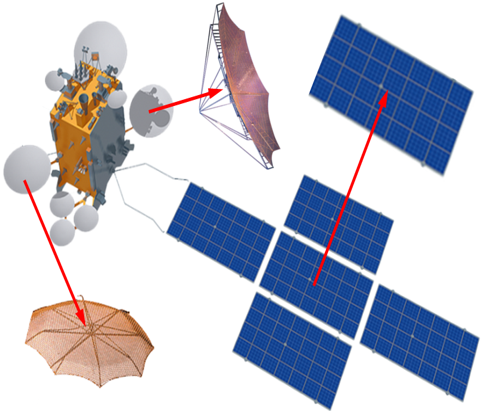
\includegraphics[width = \textwidth]{images/synopsis/decomposition}
	\end{subfigure}
	\hfill
	\begin{subfigure}[b]{0.45\textwidth}
	     % Определение стиля
        \tikzstyle{blockWide} = [rectangle, draw = black, fill = blue!15, rounded corners, text width = 20em, text centered, minimum height = 1.5em, drop shadow] 
        \tikzstyle{blockWideC} = [blockWide, fill = red!20]
        \tikzstyle{arrow} = [draw, very thick, color = black!90, line width = 0.6mm, -latex'] 
        \small
        % Задание перменных
        \def\nodeDist{0.45cm}
        % Отрисовка блок-схемы
        \begin{tikzpicture}[scale = 1, transform shape]
            % Задание узлов		
            \node (modalTests) [blockWide] {Модальные испытания \\ составных частей конструкции};
            \node (modelUpdating) [blockWide, below = \nodeDist of modalTests] {Коррекция расчетных моделей \\ составных частей  конструкции \\ по результатам испытаний};
            \node (checkInfluence) [blockWide, below = \nodeDist of modelUpdating] {Освобождение расчетных моделей \\ составных частей конструкции};
            \node (buildRealModel) [blockWide, below = \nodeDist of checkInfluence] {Синтез расчетной модели полной \\ конструкции из её составных частей};
            \node (buildMathModel) [blockWide, below = \nodeDist of buildRealModel] {Определение динамических \\ характеристик полной расчетной модели};
            % Соединение узлов
            \draw [arrow] (modalTests.south) -- (modelUpdating.north);
            \draw [arrow] (modelUpdating.south) -- (checkInfluence.north);
            \draw [arrow] (checkInfluence.south) -- (buildRealModel.north);
            \draw [arrow] (buildRealModel.south) -- (buildMathModel.north);
        \end{tikzpicture}
	\end{subfigure}
    \caption{Схема методики синтеза расчетных моделей КТК} \label{fig:schemeDecomposition}
\end{figure}  

Методика синтеза протестирована на примере модели космического аппарата, состоящего из орбитального модуля и панелей солнечных батарей. Модели каждой составной части корректировались по девяти частотам собственных колебаний, соответствующих двум виртуальным экспериментам. Распределение изменений узловых жесткостей по всем линейным степеням свободы для моделей составных частей после коррекции показано на рисунке~\ref{fig:test-spacecraft-distribution}. Максимальная погрешность в определении первых шестнадцати частот синтезированной (глобальной) модели до коррекции равнялась $ 5.1 $ \%, а после коррекции составила $ 0.1 $ \%~\tabref{tab:resultUpdatingTestSpacecraft}. 
\vspace{-0.5em}
\begin{figure}[H]
	\centering
	\begin{subfigure}[t]{0.41\textwidth}
		\centering
		\includegraphics[width = \textwidth]{test-spacecraft-orbital-distribution}
		\caption{Орбитальный модуль} \label{subfig:test-orbital-distribution}
	\end{subfigure}
	\qquad
	\begin{subfigure}[t]{0.39\textwidth}
		\centering
		\includegraphics[height = \textwidth]{test-spacecraft-panel-distribution}
		\caption{Панели солнечных батарей} \label{subfig:test-panel-distribution}
	\end{subfigure}
	\vspace{0.7em}
	\caption{Изменения жесткостей при коррекции моделей составных частей} \label{fig:test-spacecraft-distribution} 
\end{figure}

\begin{figure}[!htb]
	\centering
	\begin{minipage}{0.52\textwidth}
		\hspace{2em} Сходимость алгоритма коррекции оценивалась по частотному критерию $ \lVert \mat{\alpha} \rVert_{\max} $, равному наибольшему относительному отклонению расчетных частот от целевых значений~\figref{fig:test-spacecraft-convergence}.
		\vspace{-1.5em}
		\begin{center}
			\begin{tikzpicture}[scale = 1]
				\begin{semilogyaxis}[
					xlabel            = {Номер итерации коррекции},
					ylabel            = {$ \lVert \mat{\alpha} \rVert_{\max} $}, 
					ylabel shift      = -5 pt,
					width             = 9cm,
					grid              = both,
					legend cell align = left,
					legend style      = {
						at            = {(0.02, 0.12)},
						anchor        = west,
						fill          = white,
						fill opacity  = 0.6,
						draw opacity  = 1,
						text opacity  = 1,
					},
					ylabel near ticks,
					xmin = 0, xmax = 8
				]
					\addplot table {images/partModelUpdating/test-spacecraft-panels-convergence.txt};
					\addplot table {images/partModelUpdating/test-spacecraft-orbital-convergence.txt};
					\legend{Панели солнечных батарей, Орбитальный модуль}
				\end{semilogyaxis}
			\end{tikzpicture}
			\caption{Оценка сходимости коррекции} \label{fig:test-spacecraft-convergence}
		\end{center}
	\end{minipage}
	\hfill
	\begin{minipage}{0.45\textwidth}
		\centering
		\vspace{0.1em}
		\begin{talltblr}[
			caption = {Cинтез модели КА},
			label = {tab:resultUpdatingTestSpacecraft}
		]{
			colspec = {|X[c, -1]|X[c]|X[c]|X[c]|X[c]|},
			hlines,
			colsep = 1pt,
			rows = {font = \small}
		}
			\SetCell[r = 3]{c} Тон & \SetCell[c = 4]{c} Погрешность в частотах, \% &&& \\
			& \SetCell[r = 2]{c} Исходная & \SetCell[c = 3]{c} Коррекция по девяти частотам && \\
			& & Панелей & Модуля & {Панелей \\ и модуля} \\ \hline
			7 & -4.689 & -2.120 & -2.756 & -0.021 \\
			8 & -4.678 & -2.078 & -2.782 & -0.018 \\
			9 & -5.121 & -4.447 & -0.674 & 0.100  \\
			10 & -5.040 & -4.760 & -0.354 & -0.028 \\
			11 & -5.040 & -4.760 & -0.357 & -0.032 \\
			12 & -5.121 & -4.443 & -0.687 & 0.091 \\
			13 & -4.102 & -0.966 & -3.161 & 0.011 \\
			14 & -4.112 & -0.999 & -3.135 & 0.016 \\
			15 & -3.303 & -0.234 & -3.066 & -0.006 \\
			16 & -3.303 & -0.234 & -3.066 & -0.005 \\
		\end{talltblr}
	\end{minipage}
	\vspace{0.3em}
\end{figure}

\vspace{-0.5em}

\begin{wrapfigure}[15]{r}{0.6\textwidth}
	\centering
	\vspace{-0.25em}
	\includegraphics[width = 1\linewidth]{gencalc-interface-scaled}
	\caption{Определение модальных параметров} \label{fig:gencalc-interface}
\end{wrapfigure}

\pdfbookmark[1]{Глава 3. Результаты модальных испытаний как исходные данные для коррекции расчетных моделей конструкций}{partModalAnalysis}

\highlight{В третьей главе} развиты методы классического и операционного модального анализа, позволяющие получать достоверные оценки динамических параметров для коррекции. С целью обеспечения возможности оперативного расчета обобщенных характеристик в ходе модальных испытаний, составлена программная реализация, позволяющая посредством графического интерфейса~\figref{fig:gencalc-interface} варьировать параметры расчета и исследовать зависимости получаемых характеристик несколькими способами одновременно. Оценка качества выделения тона колебаний осуществляется построением параметра монофазности и частотного годографа колебательной системы.

Одним из ключевых требований обеспечения непрерывности производственного процесса авиационной техники является сокращение времени между натурными испытаниями и первым вылетом. Этой цели служит разработанная программа~\figref{fig:analyzer-interface}, использующая программный интерфейс \name{Testlab Automation} для обработки и представления результатов модального анализа непосредственно в процессе испытаний.

\begin{wrapfigure}[14]{r}{0.6\textwidth}
	\centering
	\includegraphics[width = \linewidth]{analyzer-interface-scaled}
	\caption{Экспресс-представление результатов} \label{fig:analyzer-interface}
\end{wrapfigure}

Изложена методика контроля зазоров в технических изделиях по искажениям портретов вынужденных колебаний в процессе вибрационных испытаний. Представлен способ поэтапного выявления всех зазоров в объекте испытаний, которые приводят к искажениям портретов колебаний. В рамках описываемого подхода разработана и интегрирована в программное обеспечение управления испытаниями программа анализа портретов колебаний. Методика обнаружения дефектов по искажениям портретов колебаний использована для диагностирования самолётов в процессе модальных испытаний~\figref{fig:distortion-wiring-backlash}, а также космических аппаратов открытого исполнения в технологических вибрационных испытаниях~\figref{fig:distortion-spacecraft}. 

\begin{figure}[!htb]
	\centering
	\begin{minipage}{0.59\textwidth}
		\centering
		\includegraphics[width = \linewidth]{distortion-wiring-backlash} 
		\captionof{figure}{Люфт в соединении ручки управления с проводкой} \label{fig:distortion-wiring-backlash}
	\end{minipage}
	\hfill
	\begin{minipage}{0.4\textwidth}
		\centering
		\includegraphics[width = 0.8\linewidth]{distortion-spacecraft}
		\captionof{figure}{Зазоры в узлах установки солнечных батарей} \label{fig:distortion-spacecraft}
	\end{minipage}
	\vspace{0.5em}
\end{figure}

\begin{wrapfigure}[10]{r}{0.5\textwidth}
	\begin{center}
		\vspace{-1.4em}
		\includegraphics[width = 1\linewidth]{reflector-experiment}
		\caption{Испытания рефлектора КА} \label{fig:reflector-experiment}
	\end{center}
\end{wrapfigure}

Разработан способ определения модальных параметров, обладающий низкий чувствительностью к дрейфу показаний (тренду) акселерометров, регистрирующих отклики конструкции на импульсное воздействие (\name{ADA}). При этом разметка по времени анализируемых участков осуществляется автоматически методом сегментации. Методы операционного модального анализа: \name{SSI}, \name{ERA}, \name{N4SID} и \name{ADA}, протестированы на примере имитационной модели беспилотного летательного аппарата и применены для определения модальных характеристик рефлектора КА по результатам испытаний в акустической камере~\figref{fig:reflector-experiment}. Исследована устойчивость значений определяемых модальных характеристик в зависимости от продолжительности записи и частоты дискретизации сигналов.

\begin{wrapfigure}[15]{r}{0.5\textwidth}
	\begin{center}
		\vspace{-2em}
		\hspace{-1em}
		\begin{tikzpicture}[scale = 1]
			\small
			\begin{axis}[
				xlabel            = {$ v $, км/ч},
				ylabel            = {$ \delta $},
				ylabel shift      = -2 pt,
				y dir             = reverse,
				grid              = major,
				legend columns    = 1,
				legend cell align = {left},
				legend style      = {
					at            = {(0.025, 0.76)},
					anchor        = west,
					fill          = white,
					fill opacity  = 0.6,
					draw opacity  = 1,
					text opacity  = 1,
				},
				ylabel near ticks,
				ymin = 0,
				x tick label style = {
					/pgf/number format/.cd,
					set thousands separator = {},
					fixed
				},
				y tick label style = {
					/pgf/number format/.cd,
					fixed
				},
				ylabel near ticks,  
				try min ticks    = 6,
				mark size        = 1.25pt,
				width            = 9cm,
				height           = 8.25cm,
			]
				\pgfplotstableread{images/synopsis/flight-decrements-2.txt}\contentFile
				\addplot[color = blue, thick, mark = *, smooth, tension = 0.2] table [x index = 0, y index = 1] {\contentFile};
				\addplot[color = gray, thick, mark = triangle*, smooth, tension = 0.2] table [x index = 0, y index = 2] {\contentFile};
				\addplot[color = teal, thick, mark = diamond*, smooth, tension = 0.2] table [x index = 0, y index = 3] {\contentFile};
				\addplot[color = red, thick,  mark = halfcircle*, smooth, tension = 0.2] table [x index = 0, y index = 4] {\contentFile};
				\addplot[color = orange, thick, densely dashed, mark = o, mark options = {solid}, smooth, tension = 0.2] table [x index = 0, y index = 5] {\contentFile};
				\addplot[color = violet, thick, densely dashed, mark = o, mark options = {solid}, smooth, tension = 0.2] table [x index = 0, y index = 6] {\contentFile};
				\legend{\name{SSI-DD}, \name{ERA}, \name{ADA}, \name{N4SID}, {\name{ЛИИ}, оценка сверху}, {\name{ЛИИ}, оценка снизу}}
			\end{axis}
		\end{tikzpicture}
		\caption{Скоростные зависимости логарифмического декремента} \label{fig:flight-decrements}
	\end{center}
\end{wrapfigure}

Получены оценки динамических параметров по результатам летных испытаний в ходе которых записывались отклики на управляемое внешнее воздействие при полете самолёта на разных скоростных режимах $ v $. Определенные после обработки и обобщения значения частот и логарифмических декрементов $ \delta $~\figref{fig:flight-decrements} являются исходными данными для исследования аэроупругой устойчивости. Для оценки корректности обработки проведено сопоставление результатов с данными летно-исследовательского института имени М.\,М.~Громова~(ЛИИ). 

\pdfbookmark[1]{Глава 4. Решение практических задач коррекции расчетных моделей}{partAprobation}

\highlight{Четвертая глава} посвящена применению разработанных методик для решения практических задач коррекции, освобождения и синтеза расчетных динамических моделей. Разработан способ моделирования податливости закреплений в условиях эксперимента. 

\begin{wrapfigure}[22]{r}{0.5\textwidth}
	\begin{center}
		\vspace{-3em}
		\includegraphics[width = 1\linewidth]{tu-204-experiment}
		\caption{Общий вид ДПМ} \label{fig:tu-204-experiment}
		\vspace{1em}
		\begin{talltblr}[
			caption = {Результаты коррекции ДПМ},
			label   = {tab:updatingTu204}
		]{
			colspec = {|c|c|c|c|c|c|c|c|},
			hlines,
			colsep = 7pt,
			rows = {font = \small}
		}
			\SetCell[r = 3]{c} Тон & \SetCell[c = 7]{c} {Погрешность до и после коррекции, \%}  \\
			& \SetCell[r = 2]{c} До & \SetCell[c = 6]{c} После \\ 
			& & 1 & 2 & 3 & 4 & 5 & 6 \\ \hline
			1 & 1.5 & 0.0 & 0.0 & 0.0 & 0.0 & 0.0 & 0.0 \\
			2 & 1.7 & -0.6 & 0.0 & 0.0 & 0.0 & 0.0 & 0.0 \\
			3 & 5.3 & 4.7 & 4.7 & 0.0 & 0.0 & 0.0 & 0.0 \\ 
			4 & 4.2 & 3.5 & 3.3 & 2.6 & 0.0 & 0.0 & 0.0 \\
			5 & -1.8 & -4.4 & -3.2 & -3.9 & -4.4 & 0.0 & 0.0 \\
			6 & 4.2 & 3.7 & 3.8 & 3.4 & 2.0 & 3.3 & 0.0 \\
		\end{talltblr}
	\end{center}
\end{wrapfigure}

Методика коррекции апробирована на динамически-подобной модели (ДПМ) самолёта \mbox{Ту-204}, выполненной по отсечно-балочной схеме. Для проведения экспериментального модального анализа ДПМ была вывешена на упругой подвеске малой жесткости~\figref{fig:tu-204-experiment}. Средствами \name{Ansys} создана КЭ-модель, имеющая $ 752 $ тысячи степеней свободы. Коррекция КЭ-модели проводилась по шести наборам, состоящих из экспериментально определенных частот. Каждый последующий набор дополнял предыдущий одним тоном собственных колебаний. Итерационный процесс коррекции завершался при достижении целевых значений частот с точностью $0.0001$\,\%. Результаты коррекции сведены в таблице~\ref{tab:updatingTu204}.

Осуществлен синтез глобальной модели каркаса зонтичной антенны по результатам испытания её составных частей. Податливость закрепления одной из составных частей в ходе экспериментов смоделирована упругими элементами, параметры которых определены на основе данных дополнительных статических испытаний. В результате проведенных исследований показано, что использование полноразмерных моделей составных частей является предпочтительным по отношению к редуцированным моделям в силу того, что первые более полно описывают связи между подконструкциями. 

\begin{wrapfigure}[14]{r}{0.5\textwidth}
	\begin{center}
		\vspace{-3em}
		\includegraphics[width = \linewidth]{wing-experiment} 
		\captionof{figure}{Общий вид ОЧК} \label{fig:wing-experiment}
	\end{center}
\end{wrapfigure}

Выполнена коррекция расчетной модели отъемной части крыла (ОЧК) изделия \mbox{С-70}~\figref{fig:wing-experiment}. По результатам экспериментального модального анализа было выявлено, что полученные частоты собственных колебаний консоли крыла существенно отличаются от расчетных. Это во многом обусловлено тем, что масса конструкции, выполненной из композиционных материалов, в расчетной схеме представлялась дискретно, а жесткостное распределение моделировалось невесомыми панелями с изотропными характеристиками. \mbox{Однако}, даже в случае столь существенных различий в схематизации, целевые частоты по пяти тонам собственных колебаний были достигнуты с заданной точностью. 

\begin{wrapfigure}[13]{r}{0.5\textwidth}
	\begin{center}
		\vspace{-1.25em}
		\includegraphics[width = \linewidth]{girder-full-system} 
		\captionof{figure}{Гирдер с оборудованием} \label{fig:girder-experiment}
	\end{center}
\end{wrapfigure}

Уточнены упругие характеристики модели гирдера (подставки), который используется для размещения электрофизического оборудования в накопительной части кольца центра коллективного пользования <<Сибирский кольцевой источник фотонов>>~\figref{fig:girder-experiment}. Коррекция позволит улучшить эксплутационные характеристики совместной системы гирдера с оборудованием за счет избежания возникновения резонансов от сейсмических колебаний, приводящих к потере качества электронного пучка. По результатам экспериментальных исследований установлено, что формы собственных колебаний, соответствующие низшим тонам, происходят при совместном перемещении гирдера и блока фундамента, на который опираются регулируемые опоры. Поэтому построена модель фундамента, идентифицированная по пяти частотам собственных колебаний, соответствующих этим движениям. Затем модель гирдера на упругом основании скорректирована по шести частотам упругих тонов собственных колебаний. Наибольшие изменения узловых жесткостей достигались в местах сопряжения конструктивных элементов гирдера. Длительность коррекции расчетной модели гирдера, обладающей $ 304 $ тысячами степеней свободы, составила $ 14 $~минут. Результаты коррекции сведены в таблице~\ref{tab:girder-results}. Минимальный критерий модального соответствия, связывающий формы колебаний до и после коррекции, равнялся $ 0.941 $~\figref{fig:girder-mac}. Суммарные модальные эффективные массы корректируемых тонов колебаний по направлениям глобальной системы координат составили: $ 79 $, $ 96 $ и $ 97 $ \%. 

\begin{figure}[!htb]
	\centering
	\begin{minipage}{0.49\textwidth}
		\begin{talltblr}[
			caption = {Коррекция модели гирдера}, 
			label = {tab:girder-results}
		]{
			colspec = {|X[c, -1]|X[c, 1.3]|X[c]|X[c]|X[c]|}, 
			hlines,
			colsep = 1pt,
			rows = {font = \small}
		}
			\SetCell[r = 2]{c} Тон & \SetCell[c = 2]{c} Частота, Гц && \SetCell[c = 2]{c} {Погрешность до и \\ после коррекции, \%} \\
			& Эксперимент & Исходная модель & До & После \\ \hline
			6 & 119.51 & 135.08 & 13.03 & \SetCell[r = 6]{c} 0.00 \\
			7 & 140.97 & 146.46 & 3.89 &  \\
			8 & 148.13 & 160.07 & 8.06 &  \\
			9 & 189.65 & 210.48 & 10.98 & \\
			10 & 197.53 & 214.18 & 8.43 & \\
			11 & 242.24 & 253.51 & 4.65 & \\
		\end{talltblr}
	\end{minipage}
	\hfill
	\begin{minipage}{0.5\textwidth}
		\centering
		\includegraphics[width = \linewidth]{girder-mac-scaled}
		\captionof{figure}{Сравнение форм колебаний} \label{fig:girder-mac}
	\end{minipage}
\end{figure}
	
	% Заключение
	
\pdfbookmark{Заключение}{conclusion}
\section*{Заключение}


\begin{enumerate}
	\item Разработана методика коррекции конечно-элементных моделей летательных аппаратов по результатам модальных испытаний, основанная на дополнении исходной модели корректирующими конечными элементами.
	\item Исследования сходимости алгоритма и чувствительности методики коррекции расчетных моделей показали, что результаты коррекции устойчивы к погрешностям эксперимента. 
	\item Разработан способ определения собственных частот и форм колебаний свободной конструкции по результатам испытаний этой конструкции с наложенными связями.
	\item Развита методика расчетно-экспериментального модального анализа конструкций по результатам испытаний их составных частей. Разработана программа и обоснованы граничные условия в испытаниях составных частей. Создано программное обеспечение, реализующее полный цикл операций для решения задачи синтеза глобальных расчетных моделей из скорректированных моделей составных частей.
	\item Формирование глобальной матрицы демпфирования конструкций по результатам испытаний их составных частей осуществляется в несколько этапов: по соотношениям между вынужденными монофазными и собственные колебаниями подтверждается диагональный вид матриц демпфирования составных частей в главных координатах, определяются обобщенные характеристики демпфирования. На основании гипотезы Е.\,С.~Сорокина строятся начальные приближения матриц демпфирования составных частей в физической системе координат. Эти матрицы уточняются решением задачи коррекции. Формирование глобальной матрицы осуществляется посредством ассемблирования матриц демпфирования составных частей. 
	\item С целью получения исходных данных для коррекции создан комплекс программ, позволяющий проводить обработку и представление результатов модального анализа непосредственно в процессе испытаний. Разработано программное обеспечение для контроля параметров технического состояния изделий в процессе испытаний.
	\item Эффективность разработанных методик и программного обеспечения подтверждена результатами решения практических задач коррекции расчетных моделей конструкций.
\end{enumerate}

\textbf{Рекомендации и перспективы дальнейшей разработки темы}

Перспективным направлением дальнейших исследований является развитие разработанных вычислительных алгоритмов для ускорения сходимости в задачах коррекции. Это особенно актуально при коррекции расчетных моделей с высокой степенью детализации. Было отмечено, что обобщенное отношение Рэлея отличается от значений собственных чисел, получаемых при решении обобщенной проблемы собственных значений. Причина состоит в численных округлениях при расчете собственных форм колебаний с нулевыми собственными значениями.

Прикладной аспект дальнейшей работы выражается в создании вспомогательных программ, позволяющих учитывать информацию о корректирующих элементах в конечно-элементных пакетах, использованных для создания исходных моделей. Это обеспечит взаимодействие встроенными средствами со скорректированными расчетными моделями, в том числе их применение для решения задач вынужденных колебаний и нелинейной динамики.

Перспективным также является создание программного обеспечения для контроля параметров технического состояния изделий по эксплуатационным вибрациям.

	% Публикации
	
\newcommand{\listPublications}{\pdfbookmark[0]{Список основных научных публикаций по теме диссертации}{listPublications}\textbf{Список основных научных публикаций по теме диссертации}}

{\listPublications}

\ul{Статьи в рецензируемых научных изданиях, входящих в список ВАК, в том числе, входящих в международные реферативные базы данных:}

\begin{enumerate}
	\item Метод коррекции конечно-элементных моделей динамических систем~/ Д.\,А.~Красноруцкий, П.\,А.~Лакиза, В.\,А.~Бернс, Е.\,П.~Жуков // Вестник Пермского национального исследовательского политехнического университета. Механика.~--- 2021.~--- №~3.~--- С.~84--95. 
	\item Контроль зазоров в конструкциях технических изделий в процессе вибрационных испытаний~/ Н.\,А.~Тестоедов, В.\,А.~Бернс, Е.\,П.~Жуков,
Е.\,А.~Лысенко, П.\,А.~Лакиза~// Обработка металлов (технология, оборудование, инструменты).~--- 2021.~--- Т.~23, №~2.~--- С.~40--53.
	\item Метод освобождения динамической расчетной модели летательного аппарата~/ Д.\,А.~Красноруцкий, В.\,А.~Бернс, П.\,А.~Лакиза, В.\,Е.~Левин~// Научный журнал <<Известия Самарского научного центра РАН>>.~--- 2019.~--- Т.~21, №~1.~--- С.~31--38.
	\item Исследования достоверности диагностирования трещин по искажениям портретов вынужденных колебаний / В.\,А.~Бернс, Е.\,П.~Жуков, П.\,А.~Лакиза, E.\,А.~Лысенко // Обработка металлов (технология, оборудование, инструменты).~--- 2019.~--- Т.~21, №~2.~--- С.~26--39.
\end{enumerate}

\ul{Патент на изобретение в РФ:}

\begin{enumerate}
	\item Пат.~2728329 Российская Федерация, МПК G01M7/00. Способ определения собственных частот и форм колебаний свободной конструкции по результатам испытаний этой конструкции с наложенными связями~/ Бернс~В.\,А., Жуков~Е.\,П., Красноруцкий~Д.\,А., Лакиза~П.\,А.~--- № 2019119278; заявл.~19.06.19; опубл.~29.06.20, Бюл.~№ 22.~--- 15~с.
\end{enumerate}

\ul{Свидетельства о государственной регистрации программ для ЭВМ:}

\begin{enumerate}
	\item Свидетельство 2023610282. Операционный модальный анализ летательных аппаратов <<FlightLab>>: программа для ЭВМ~/ П.\,А.~Лакиза, Д.\,А.~Красноруцкий, В.\,А.~Бернс (RU); правообладатель <<Новосибирский государственный технический университет>>; заявл.~10.01.2023; опубл.~10.01.2023.
	\item Свидетельство 2021663099. Контроль дефектов в процессе вибрационных испытаний <<DistortionFinder>>: программа для ЭВМ / П.\,А. Лакиза, В.\,А.~Бернс, Е.\,П.~Жуков (RU); правообладатель <<Новосибирский государственный технический университет>>; заявл.~02.08.2021; опубл.~11.08.2021.
 	\item Свидетельство 2021662816. Представление результатов модальных испытаний <<ResponseAnalyzer>>: программа для ЭВМ / П.\,А.~Лакиза, В.\,А.~Бернс, Е.\,П.~Жуков (RU); правообладатель <<Новосибирский государственный технический университет>>; заявл.~02.08.2021; опубл.~05.08.2021.
	\item Свидетельство 2021662965. Расчет обобщенных характеристик тонов собственных колебаний по результатам модальных испытаний <<GenCalc>>: программа для ЭВМ / П.\,А.~Лакиза, В.\,А.~Бернс, Е.\,П.~Жуков (RU); правообладатель <<Новосибирский государственный технический университет>>; заявл.~02.08.2021; опубл.~10.08.2021.
\end{enumerate}

\ul{В прочих изданиях:}

\begin{enumerate}
	\item Применение операционного модального анализа для определения динамических характеристик летательных аппаратов~/ В.\,А.~Бернс, А.\,И.~Годин, Е.\,П.~Жуков, Д.\,А.~Красноруцкий, П.\,А.~Лакиза, Д.\,А.~Маринин, А.\,В.~Пара и А.\,В.~Шкода~// Материалы XXVI Международной научно-практической конференции <<Решетневские чтения>>.~--- Красноярск : СибГУ им.~М.\,Ф.~Решетнёва.~--- 9--11 ноября 2022 г.~--- Т. 1.~--- С.~90--92.
	\item К вопросу коррекции расчетных моделей летательных аппаратов~/ В.\,А.~Бернс, А.\,И.~Годин, Е.\,П.~Жуков, Д.\,А.~Красноруцкий, П.\,А.~Лакиза, Е.\,А.~Лысенко, А.\,В.~Пара и А.\,В.~Шкода~// Материалы XXVI Международной научно-практической конференции <<Решетневские чтения>>.~--- Красноярск : СибГУ им.~М.\,Ф.~Решетнёва.~--- 9--11 ноября 2022 г.~--- Т.~1.~--- C.~87--89.
	\item Коррекция расчетной модели отъемной части крыла летательного аппарата~/ В.\,А.~Бернс, А.\,И.~Годин, Е.\,П.~Жуков, Д.\,А.~Красноруцкий, П.\,А.~Лакиза и А.\,В.~Пара~// Материалы 6-ой международной научно-технической конференции <<Динамика и виброакустика машин>> (DVM 2022).~--- Самара : Самарский университет.~--- 21--23 сентября 2022 г.~--- C. 217--219.
	\item Использование портретов колебаний в процессе контроля технического состояния летательных аппаратов~/ В.\,А.~Бернс, Е.\,А.~Лысенко, Е.\,П.~Жуков, П.\,А.~Лакиза и Д.\,О.~Душухин~// Общероссийский научно-технический журнал <<Полёт>>.~--- 2022.~--- №~2.~--- C.~64--71.
	\item Результаты модальных испытаний как исходные данные для коррекции расчетных моделей летательных аппаратов~/ В.\,А.~Бернс, Е.\,П.~Жуков, П.\,А.~Лакиза, Маленкова В. В. и Д.\,О.~Душухин~// Общероссийский научно-технический журнал <<Полёт>>.~--- 2022.~--- №~2.~--- C.~49--56.
	\item Метод коррекции расчетных динамических моделей летательных аппаратов~/ Д.\,А.~Красноруцкий, В.\,А.~Бернс, П.\,А.~Лакиза, Е.\,П.~Жуков и Д.\,А.~Маринин~// Материалы XXV Международной научно-практической конференции <<Решетневские чтения>>.~--- Красноярск : СибГУ им.~М.\,Ф.~Решетнёва.~--- 10--12 ноября 2021 г.~--- Т.~1.~--- C.~94--95.
	\item Идентификация дефектов в конструкциях летательных аппаратов по портретам вынужденных колебаний~/ В.\,А.~Бернс, Е.\,А.~Лысенко, Е.\,П.~Жуков и П.\,А.~Лакиза~// Материалы XXV Международной научно-практической конференции <<Решетневские чтения>>.~--- Красноярск : СибГУ им.~М.\,Ф.~Решетнёва.~--- 10--12 ноября 2021 г.~--- Т.~1.~--- C.~69--70.
	\item Control of Defects in Airframes during Ground Vibration Testing~/ V.\,A.~Berns, E.\,A.~Lysenko, E.\,P.~Zhukov, P.\,A~Lakiza~// Fundamental Problems of Aircraft Aerodynamics, Flight Dynamics, Strength and Flight Safety. Proceedings 7-th Russian-Chinese Conference.~--- Zhukovsky.~--- 11--14 October 2021.~--- P. 71--72.
	\item A Method for Finite Element Model Updating of Aircraft Based on Ground Vibration Testing Results~/ D.\,A.~Krasnorutsky, V.\,A.~Berns, E.\,P.~Zhukov, P.\,A.~Lakiza~// Fundamental Problems of Aircraft Aerodynamics, Flight Dynamics, Strength and Flight Safety. Proceedings 7-th Russian-Chinese Conference.~--- Zhukovsky.~--- 11--14 October 2021.~--- P. 65--66.
	\item Использование портретов колебаний в контроле технического состояния летательных аппаратов~/ В.\,А.~Бернс, Е.\,А~Лысенко, Е.\,П.~Жуков, П.\,А.~Лакиза~// Материалы школы-семинара <<Проблемы прочности авиационных конструкций и материалов>>.~--- Новосибирск.~--- 8~--~11 сентября 2021 г.~--- C.~14--15.
	\item Результаты модальных испытаний как исходных данные для коррекции расчетных моделей летательных аппаратов~/ В.\,А.~Бернс, Е.\,П.~Жуков, П.\,А.~Лакиза, В.\,В~Маленкова~// Материалы школы-семинара <<Проблемы прочности авиационных конструкций и материалов>>.~--- Новосибирск.~--- 8--11 сентября 2021 г.~--- С.~12--14.
	\item Разработка метода коррекции динамических конечно-элементных моделей по результатам частотных испытаний~/ П.\,А.~Лакиза, Д.\,А~Красноруцкий, В\,А.~Бернс, Е.\,П.~Жуков~// Труды Всероссийской научной конференции молодых ученых <<Наука. Технологии. Иновации>>.~--- Новосибирск : Изд-во НГТУ.~--- 30 ноября~--~4 декабря 2020 г.~--- Т.~9.~--- C.~23--26.
	\item Лакиза~П.\,А. Разработка метода синтеза математических моделей крупногабаритных трансформируемых космических конструкций по результатам испытаний их составных частей~// Материалы 58-й Международной научной студенческой конференции МНСК-2020: Математика.~--- 2020.~--- C.~124.
	\item Лакиза~П.\,А., Красноруцкий~Д.\,А. Метод коррекции математических моделей, полученных путем конечно-элементного моделирования~// Труды Всероссийской научной конференции молодых ученых <<Наука. Технологии. Иновации>>.~--- 2019.~--- Т.~9.~--- C.~57--59.
	\item О возможности модальных испытаний самолётов на жёстких опорах~/ Э.\,А.~Занина, В.\,А.~Бернс, П.\,А.~Лакиза~// Труды Всероссийской научной конференции молодых ученых <<Наука. Технологии. Иновации>>.~--- Новосибирск : Изд-во НГТУ.~--- 2019.~--- Т.~9.~--- C.~45--48.
	\item Расчетно-экспериментальный метод модального анализа крупногабаритных трансформируемых конструкций~/ В.\,А.~Бернс, Д.\,А.~Красноруцкий, П.\,А.~Лакиза, Д.\,А.~Маринин, Е.\,П.~Жуков~// Материалы XXIII Международной научно-практической конференции <<Решетневские чтения>>.~--- Красноярск : СибГУ им. М. Ф. Решетнёва.~--- 11--15 ноября 2019 г.~--- Т.~1.~--- C.~82--83.
	\item Lakiza~P.\,A., Krasnorutskiy~D.\,A. A Method for Updating Mathematical Models Obtained by Finite-Element Modelling~// Progress through innovations. Proceedings 2019 VIII-th International Academic and Research Conference of Graduate and Postgraduate Students.~--- Novosibirsk : Nstu pub.~--- 2019.~--- P.~151--153.
	\item Development of a Calculation Method for Modal Analysis of Large Transformable Space Structures~/ P.\,A.~Lakiza, D.\,A.~Krasnorutskiy, M.\,D.~Golysheva ~// Science. Research. Practice. Proceedings 2018 IInd All Russia Academic and Research Conference of Graduate and Postgraduate Students.~--- Novosibirsk : Nstu pub.~--- 2019.~--- P. 76--78.
	\item Разработка расчетно-экспериментального метода модального анализа крупногабаритных трансформируемых космических конструкций~/ В.\,А.~Бернс, В.\,Е.~Левин, Д.\,А.~Красноруцкий, Д.\,А.~Маринин, Е.\,П.~Жуков, В.\,В.~Маленкова, П.\,А.~Лакиза~// Научный журнал <<Космические аппараты и технологии>>.~--- 2018.~--- C.~125--133.
	\item Исследование способа выявления трещин по портретам вынужденных колебаний~/ В.\,А.~Бернс, Е.\,П.~Жуков, Е.\,А.~Лысенко, В.\,В.~Маленкова, П.\,А.~Лакиза~// Материалы XXII Международной научно-практической конференции <<Решетневские чтения>>.~--- Красноярск : СибГУ им.~М.\,Ф.~Решетнёва.~--- 12--16 ноября 2018 г.~--- Т.~1.~--- C.~82--83.
	\item Модальный анализ макета антенны космического аппарата по результатам испытаний его составных частей~/ В.\,А.~Бернс, В.\,Е.~Левин, Д.\,А.~Красноруцкий, Е.\,П.~Жуков, П.\,А.~Лакиза~// Материалы XXII Международной научно-практической конференции <<Решетневские чтения>>.~--- Красноярск : СибГУ им. М. Ф. Решетнёва.~--- 12--16 ноября 2018 г.~--- Т.~1.~--- C.~84--85.
	\item Контроль дефектов конструкций летательных аппаратов по портретам вынужденных колебаний~/ В.\,А.~Бернс, Е.\,П.~Жуков, П.\,А.~Лакиза и В.\,В.~Маленкова~// Материалы XXIV Международного симпозиума <<Динамические и технологические проблемы механики конструкций и сплошных сред>> имени А.\,Г.~Горшкова.~--- М. : ООО <<ТРП>>.~--- 2018.~--- Т.~1.~--- C.~45--47.
	\item Диагностика процессов разрушения элементов конструкций летательных аппаратов~/ В.\,А.~Бернс, Е.\,П.~Жуков, Е.\,А.~Лысенко, В.\,В.~Маленкова и П.\,А.~Лакиза~// Материалы XXI Международной научно-практической конференции <<Решетневские чтения>>.~--- Красноярск : СибГУ им.~М.\,Ф.~Решетнёва.~--- 08--11 ноября 2017 г.~--- Т.~1.~--- C.~84--86.
\end{enumerate}
	
	% Типография
	
\newpage
\thispagestyle{empty}
\vspace*{0pt plus1fill}
\begin{center}
    \textit{Лакиза Павел Анатольевич}
    \par\smallskip

    Коррекция расчетных моделей летательных аппаратов 
    по результатам \par модальных испытаний
    \par\smallskip

    Автореферат диссертации на соискание ученой степени \par
    кандидата технических наук
    \par\medskip
    
    Отпечатано в типографии \par
    Новосибирского государственного технического университета \par   
    630073, г.~Новосибирск, пр.~К.~Маркса, 20 \par
    Тел.\,/\,факс: (383)\,346-08-57 \par
    Подписано в печать 10.04.2023 г. Заказ № \fixme{9999}. \par
    Формат 60$\times$84 1/16. Объем 1.25 п.л. Тираж 100 экз.
\end{center}
\end{document}
